\chapter{Charting Deep-Sea Hydrothermal Plumes in the Field}
\label{chap:field_results}

\begin{center}
    \begin{minipage}{0.7\textwidth}
      \begin{small}
      I had a blank canvas to fill with extraordinary possibilities, a fascinating jigsaw puzzle to piece together: mapping the world's vast hidden seafloor.\\ \emph{Marie Tharp}
      \end{small}
    \end{minipage}
    \vspace{0.5cm}
\end{center}

In this chapter, we examine how the autonomy tools \PHORTEX and \PHUMES support a real \emph{deployment-by-deployment} field operation in the Guaymas Basin, Gulf of California and post-expedition analysis. One of the key differentiators between robot-based experiments and field work using robots is how one can think about the data that's been generated. In robot-based experiments, data that is collected is typically designed to assist in directly assessing the efficacy of a robot platform; the environment may be engineered so the ``ground truth'' may be available (e.g., using ViCon systems, or having an eye-in-the-sky in terrestrial applications) and robotic measurements may map directly to a metric of interest to score performance. In contrast, in field settings there is typically no access to a ground truth (if there were, then perhaps there would be no need for the robotic platform), and the sensing equipment on the robot (and deployed around it) are opportunistic sensors which are often a proxy for the true phenomenon of interest. For instance, there is no ``plume-detection'' sensor; instead the binary measurement described in \cref{chap:phortex} must be approximated from a set of continuous-valued observations of temperature, salinity, chemistry with complicated interrelationships. Here, we discuss the engineering practicalities of arriving to a sensor model from scientific field data suitable for \PHUMES, using \PHORTEX to plan AUV \Sentry missions, and qualitatively comparing the performance of these trajectories with science-team designed dives. 

An additional aspect of performing fieldwork is that the data product that is created is itself a contribution in the context of the science or task that is being conducted. While analyzing the collected data after a field trial can be done agnostic to the autonomy system that collected the data, the \PHUMES model directly learns a probabilistic representation over semantically meaningful quantities---fluid velocity at the vent, vent area, and mixing coefficients. There is an opportunity then to investigate the utility of \PHUMES for scientific inquiries following a research cruise, and here we identify several queries that can be supported by the \PHUMES representation. 

Research presented in this chapter is adapted and extended from~\cite{preston2022physically}.   


\section{Introduction}
As presented in \cref{chap:phortex}, \PHORTEX (with \PHUMES embedded), is an autonomy system designed to uncover the dynamics model of spatiotemporal distributions from sparse observations, and leverage that dynamics model to plan strategically useful trajectories for AUV \Sentry to execute during non-adaptive multi-hour dives. In this formulation, it was taken for granted that a binary observation of plume presence was available as a data product for \PHUMES. Access to a binary measurement has been generally assumed in vent-hunting or source-seeking literature\autocite{tian2014behavior,saigol2009information,jakuba2007stochastic} as a means for identifying, with confidence, the buoyant stem of a plume expression, which is informative of the vent location. As established in \cref{chap:afar}, in practice there is no ``plume detector'' on an AUV, and so this measurement must be approximated from continuous measurements from multiple science sensors. This lack of exact sensing is due to the variable values of temperature, chemistry, and particulate matter that persist within a plume structure. In the buoyant stem of a plume, positive temperature anomalies may be several degrees warmer compared to ambient seawater; however in the neutrally-buoyant plume layer, these anomalies may be on the scale of sensor noise (only a few hundredths of a degree). Chemistry anomalies may persist longer within a plume, but are subject to unknown and variable rates of microbial digestion or chemical reaction with the environment. Moreover, some chemical signatures may not specifically fingerprint hydrothermal anomalies, and could be equally indicative of other water-mass mixing events in the deep ocean. Additionally, some oceanographic properties (e.g., temperature) vary in the water column as a function of depth, and so data must be detrended with respect to position in the water column. Taken together, the environmental complexity requires developing a sensing strategy that can fuse observations from multiple science sensors onboard AUV \Sentry into a data product that indicates whether the robot encountered hydrothermal plume fluids. In \cref{sec:field_sensor_models}, we present a method for processing standard scientific equipment on AUV \Sentry into a binary measurement that can successfully identify both buoyant stem and neutrally-buoyant plume detections for plume charting.

Separately, binary measurements are not easily informative of other types of structure useful for formulating the \PHUMES predictive model. For instance, the current transition function, $T_c$, could potentially be approximated from binary observations, but it would be significantly more straightforward if even point measurements of current magnitude and heading were available. Opportunistic sensor deployments, or leveraging the continuous value of some onboard sensors, may be one key way of alleviating the burden on the binary detections alone within the \PHUMES inference framework. Opportunistic sensor deployments are science party activities which yield data products that can be widely applicable across projects. For current, it is not atypical for an AUV to be equipped with acoustic equipment that can record water column velocity relative to a moving robot. For the expedition we present here, this was not an available sensor to us, however, tiltmeters could be deployed by ROV \emph{JASON} on the seafloor, and these instruments could serve a similar purpose, just externally to \Sentry. The challenge then is determining how to incorporate disparate sensors neatly into \PHUMES. Focusing on data available from \emph{JASON} directly, tiltmeters, and vertical profiles conducted by the shipboard rosette, we show how \PHUMES can act as a data ``aggregator'' while at sea to ultimately assist in \Sentry mission in \cref{sec:external_current}.

The ultimate goal of utilizing \PHORTEX is to collect observations that are useful for downstream science tasks. Sample spatial diversity and temporal diversity are particularly key metrics for addressing novel questions about plume manifestation in the water column: how far do detectable anomalies travel from a vent? what is the vertical structure of the neutrally buoyant layer, and how does it evolve horizontally? how does microbial activity change within a plume structure? These questions have been historically difficult to answer using normal surveying methods, which tend to spatially cluster observations at a vent source, and rarely re-encounter a plume over time. Over four dives with AUV \Sentry, we directly estimate the performance of \PHORTEX over these metrics and compare this performance with reference expert-trajectories in \cref{sec:phortex_performance}.

One of the key pieces of intuition that enables \PHORTEX to perform well at collecting spatially and temporally diverse samples is the use of an analytical model of plume dynamics within \PHUMES. The use of idealized models such as~\cite{morton1956turbulent} or~\cite{speer1989model} for estimating heat (and other energy) fluxes from collected observations at a vent source are common in scientific publications in hydrothermalism\autocite{barreyre2012structure,wilson1996hydrothermal,mittelstaedt2012quantifying,baker1993method,ramondenc2006first}. While useful, a known limitation of these models is that they fail to consider the impact of crossflow on the observable characteristics of a plume from water column data, strictly underestimating the energetic input of vents. The model at the heart of \PHUMES explicitly considers crossflow as it strategically applies to collecting samples, and in \cref{sec:phumes_as_science} we investigate how using the \PHUMES representation can be used to perform similar energy analyses, in addition to re-constructing the turbid structure of the water column as it compares to vertical transects collected by rosette.

\paragraph{Contributions}
We demonstrate \PHORTEX with \PHUMES in field trials for hydrothermal plume charting with AUV \Sentry. In so doing, we present a method of processing real \emph{in situ} observations taken by instruments on \Sentry into a data product which can be used to indicate whether a particular observation is plume or ambient seawater. We also discuss the practicalities of using external sensing equipment available during the field trial to benefit the \PHUMES formulation. Through this field trial, we demonstrate the first iterative offline planning technique for plume charting with deep-sea capable vehicles, illustrating a novel capability for these assets for future research expeditions and putting over 75\% of known vent fields\autocite{beaulieu2013authoritative} in reach for strategic charting and surveying. In analysis of the field trial results, we investigate the quality of the scientific observations and show how the \PHUMES model enables energy estimation and neutrally-buoyant plume reconstruction capabilities, and may stand to introduce a new paradigm for analyzing scientific data from AUV, ROV, or rosette studies of hydrothermal vents.  


\section{Related Work}
\label{sec:field_rw}
\subsection{Treating Plume Observations}
Since hydrothermal vents were discovered in 1977~\autocite{corliss1979submarine}, studies of hydrothermal vents have richly explored how to describe, measure, and analyze venting structures and the plumes that they produce. Water column detections of plumes are typically shared in the context of vent field discovery and are used to describe the gross characteristics of a venting site (e.g., neutrally-buoyant intrusion height, relative chemical potency, turbidity)\footnote{e.g., \autocite{kim2020discovery,caratori2012crustal,baker2019posteruption}}. In the discovery context, an important function of water column data is to establish the location of a vent that produces the plume that is observed\footnote{e.g., \autocite{jakuba2007stochastic,branch2020demonstration, jakuba2008autonomous}}, as establishing where a vent is located can be directly compared to the bathymetry of a region, and the characteristic \emph{type} of magmatic activity or hydrothermal formation can be estimated (e.g., on-axis versus off-axis, new or established). Moreover, with a vent location, specialized equipment (like ROV \emph{JASON}) can be deployed for close study of the venting chimney source; estimating the location well keeps these operations efficient and more time can be spent at a site of interest, rather than trying to locate one.

In vent finding, there are two philosophies to approaching sensor models, which are directly tied to the type of autonomous decision-making available. In theoretical odor hunting, or terrestrial/atmospheric applications in which underway autonomy is typically available, a continuous signal of some tracer (e.g., temperature) is generally used. This signal allows a robot to myopically converge to a source\autocite{morse1998robust, edwards2005moth, reddy2022olfactory, wang20203, mason2020evaluation} or to update an inverse model for source location\autocite{vergassola2007infotaxis,salam2019adaptive}. While we've discussed that choosing a single tracer is insufficient for identifying plume water \emph{when we care about recreating the structure of a plume}, any of temperature, methane, or ORP could be used in a gradient-descent style autonomy to find a venting source in a myopic strategy. However, as the mission at hand is to survey the entire structure of a plume, actually being able to distinguish the edges of the plume from background water is important.

The second philosophical approach assumes limited or no access to autonomous behaviors, and so every observation that is collected must be considered for vent identification. A popular solution has been the development of occupancy-grid style representations\autocite{jakuba2008autonomous,peng2014dynamic}, which are updated from binary observations of whether an observation was plume-derived or not. More confident ``occupied'' regions then may correspond directly with the location of the venting plume. While we do not use an occupancy grid representation (which does not easily extend to the temporal aspect of the problem we would like to address), we adapt the binary sensor model typically used in these representations to filter our observations. In~\cite{jakuba2007stochastic}, plume fluid from hydrothermal vents is identified using temperature, turbidity, ORP, and vertical velocity anomaly\footnote{Disturbances in Z-axis acceleration according to vehicle inertial sensors.}. Temperature and turbidity are detrended using reference vertical profiles of these quantities in the field site that the AUV is deployed; all sensor streams are then processed twice---once to identify buoyant stem detections, and once to identify neutrally-buoyant plume detections. Buoyant stem detections, more indicative of the location of a vent, are identified using an outlier detection technique (Hampel identifier\autocite{liu2004line}) and a consensus scheme that requires multiple corresponding outlier detections across the sensors used. In contrast, neutrally-buoyant plume detections are identified individually and using confidence intervals computed over each data stream. The treatment of neutrally-buoyant detections in this manner is problematic for our purposes, as the method is not robust to rejecting other types of latent structure that may register as small scale anomalies---for instance, cold anomalies are just as likely to be claimed hydrothermal signatures as warm ones, and natural horizontal structure that may be present in chemical distributions (like oxygen) as a product of microbial activity sustained by plume fluids, will artificially inflate the confidence intervals to essentially render those sensors useless. In this work, we address these limitations directly in our choices for per-sensor detection, and add new types of sensing---oxygen and methane---to the detection scheme.

\subsection{Autonomous Robots Studying Hydrothermalism}
AUVs are popular tools for geological surveys and mapping of the seafloor; for hydrothermal vent studies, that these platforms can also measure geochemical signatures is largely a bonus\autocite{clague2008abundance,kumagai2010hydrothermal,kinsey2011assessing,ryan2011high,caratori2012crustal,baker2019posteruption,mcphail2010challenges,schmid2019physico}. Development and demonstration of new AUV technologies that specialize in hydrothermal studies\footnote{e.g., \autocite{maki2014auv,okamoto2019visual}} demonstrate the general interest in using AUVs for studying hydrothermal sites and extending the capabilities of these vehicles beyond traditional bathymetric mapping. Adding sophistication to the autonomy of AUVs is one such avenue of active research\autocite{branch2020demonstration,wang20203,mason2020evaluation,saigol2009information}. Notably, many of these studies either assume some agency of the AUV to adjust trajectories on the fly\autocite{branch2020demonstration,wang20203,saigol2009information} or are primarily focused on processing AUV data products post-analysis to inform the deployment of other equipment\autocite{jakuba2008autonomous}. For studies in which ``closing-the-loop'' is done via online settings, many were performed in simulation, and if deployed, were primarily done in shallow-water settings with gliding vehicles, which have distinctly different operational restrictions to AUV \Sentry. As far as we are aware, there has not been a demonstration of closed-loop trajectory design for depth-capable robots to actually study a real hydrothermal plume, and so this chapter provides a unique insight on the practicalities of enabling these missions.

\subsection{Using Observations in Scientific Discovery}
In the ocean sciences, considerable attention is paid to \emph{stuff} transfer, either from air-sea interactions or crust-ocean, where \emph{stuff} may be energy in the form of heat, chemicals, or particulates (among other things). Whenever \emph{stuff} is transferred, there is a change in the relationship between the two environments, with far-reaching implications to other systems. For instance, the ocean is estimated to absorb up to half of excess atmospheric carbon dioxide emissions from anthropogenic activities\autocite{hori2019blue,raven2005ocean}. This directly connects to estimating global climate and climate-regulation mechanisms, projecting the rate of acidification of the ocean, and modeling interventions that address atmospheric carbon loads. For deep ocean studies, understanding the load of chemical and energy influx into the deep ocean from underlying magmatic activity helps to shape our models of regulatory mechanisms in the deep sea. This in turn could lead to improved future-looking understanding of how deep sea mining, deep carbon sequestration, and similar policy and engineering activities may impact the deep biogeosphere.

To estimate energetic input, the heat flux of a vent is a useful measurement for estimating the thermal energy of a vent (thermal energy is heat flux multiplied by the area of the source vent). To compute heat flux or particulate transport, stationary models of buoyant plume rise are typically inverted, using observations of the location of a neutrally buoyant plume height or noisy absolute sensor measurements to estimate the vent parameters (if such parameters cannot be directly observed using an e.g., ROV)\autocite{barreyre2012structure,barreyre2011dispersal,wilson1996hydrothermal,mittelstaedt2012quantifying,baker1993method,ramondenc2006first,murch2020volcaniclastic}. The strict assumption that there is no effect of crossflow for estimating vent characteristics can lead to an underestimate of heat and particulate input from a vent, as crossflow tends to lower the observable neutrally-buoyant height, and increase plume entrainment of background seawater\autocite{tohidi2016highly,adams2020turbulence}. By failing to consider crossflow when analyzing water column data, there are also limits placed on the ability to reconstruct the particulate/nutrient flux and transport from a vent, in addition to the vertical-horizontal distribution and longevity of plume-derived fluids. Some studies compensate for this by applying a simple advective-diffusive model at the observed neutrally-buoyant height to model horizontal transport\autocite{barreyre2011dispersal,murch2020volcaniclastic}, however extensive laboratory studies on the impact of neutrally-buoyant intrusions\autocite{richards2014radial} have shown that there is considerable complexity in the formation and persistence of a neutrally-buoyant plume, and so these simplified models may fail to generalize well outside of specific contexts in which they are applied. We briefly investigate how \PHUMES, which embeds a notion of crossflow directly in its formulation, might enable study of the neutrally-buoyant intrusion and energetic/particular fluxes, and compare these results with vertical transects performed with a rosette during the Guaymas study. 


\section{Methods}
\label{sec:field_methods}

\subsection{Plume Detection: Treatment of AUV \Sentry Science Sensors}
\label{sec:field_sensor_models}
We elect to process the heterogeneous sensor stream into a binary measurement stream, drawing on the work in~\cite{jakuba2007stochastic}, to indicate whether \Sentry was in a plume or in background seawater. In the autonomy study, \Sentry was equipped the same instrumentation as described in \cref{sec:sentry} (i.e., temperature, salinity, oxygen, turbidity, and methane observations) in addition to an oxidation reduction potential (ORP) instrument\footnote{An ORP probe measures the relative reactivity of a water sample.} to compute a binary detection of plume water. Sensors are internally logged at variable rates, but interpolated and sub-sampled to a fixed 1 Hz frequency with a shared clock time for the purposes of directly comparing the instruments. Each of the sensors has its own characteristic response to the chemistry of plume water. For example, ORP exhibits a large negative spike when first encountering plume water followed by a slow hysteresis back to a nominal values. Measurements of salinity, temperature, and oxygen are expected to be influenced not only by plume water, but background physical mixing in the ocean\autocite{li2020increasing,speer1989model,preston2022physically}; turbidity, ORP, and methane are signals strongly associated with hydrothermalism and are generally not persistent in background seawater.

To account for the different ways in which instruments respond to plumes, each sensor is processed individually to detect anomalies (both short-lived and persistent, in the case of neutrally-buoyant plumes) in each stream (see \cref{tab:sentry_instruments}). This process is directly informed by the lessons learned in \cref{chap:afar} and to address issues in detecting neutrally-buoyant detections outlined in \cref{sec:field_rw}:
\begin{itemize}
    \item Salinity and temperature signals must be detrended due to the nontrivial density stratification in the Basin.
    \item Salinity anomalies are exceedingly small, even at a vent source, and any anomaly may be indicative of hydrothermal activity.
    \item Oxygen and temperature are susceptible to other forms of physical water mass mixing in the basin.
    \item For conservative detections, a detected temperature anomaly should be classified as hydrothermalism only if elevated.
    \item Oxygen structure is complicated in the basin, likely as a result of microbial activity. A rolling window is necessary to detect localized anomalies.
    \item Turbidity and methane are significantly and obviously elevated only near hydrothermal venting.    
\end{itemize}

Weights are assigned to each sensor based on their individual reliability for identifying plume water, as determined by the science party and consulted experts in preparation for the research expedition. An observation (a vector of continuous valued sensor observations), is then classified as either plume water or background water by computing the weighted sum of the individual sensor binary detections and setting a heuristic threshold (which serves as an ``evidence minimum''). A total corroboration score of 4 or more was used to classify an observation as plume water, which ultimately computes to a single binary measurement for each observation. An example of this sensor applied to \Sentry detections during an at-sea trial in Guaymas Basin is shown in \cref{fig:detection_example}.

\begin{table}[h!]
    \centering
    \begin{tabular}{c|p{0.6\linewidth}|c}
        Quantity & Positive Plume Detection Criteria & Weight  \\
        \hline
        Salinity & Detrended practical salinity outside 3 standard deviations of the entire time series & 1 \\
        Temperature & Detrended temperatures above the 75th percentile of entire time series & 2 \\
        ORP & Detections less than -0.005 & 2 \\
        OBS & Optical attenuation above the 75th percentile of entire time series & 2 \\
        Oxygen & Detrended concentrations outside one-hour rolling computation of 3 standard deviations & 1 \\
        Methane & Normalized concentration above 0.3 & 2
    \end{tabular}
    \caption[Instruments on AUV \Sentry and the criteria used to identify plume fluids for each instrument.]{\textbf{Instruments on AUV \Sentry and the criteria used to identify plume fluids for each instrument.} The weight is used to indicate relative trustworthiness of a plume detection for each sensor, and is used in a corroboration scheme that sums detections across sensors in order to make a final determination on whether an observation location contained a parcel of plume fluid or consisted of background seawater. Detrended data removes depth-related cross-sensitivity from the measurements; for example, temperature is stratified in the deep ocean, so to ignore the impacts of depth changes in the data stream, those effects are removed by normalizing the data with respect to depth.}
    \label{tab:sentry_instruments}
\end{table}

\begin{figure}[h!]
    \centering
    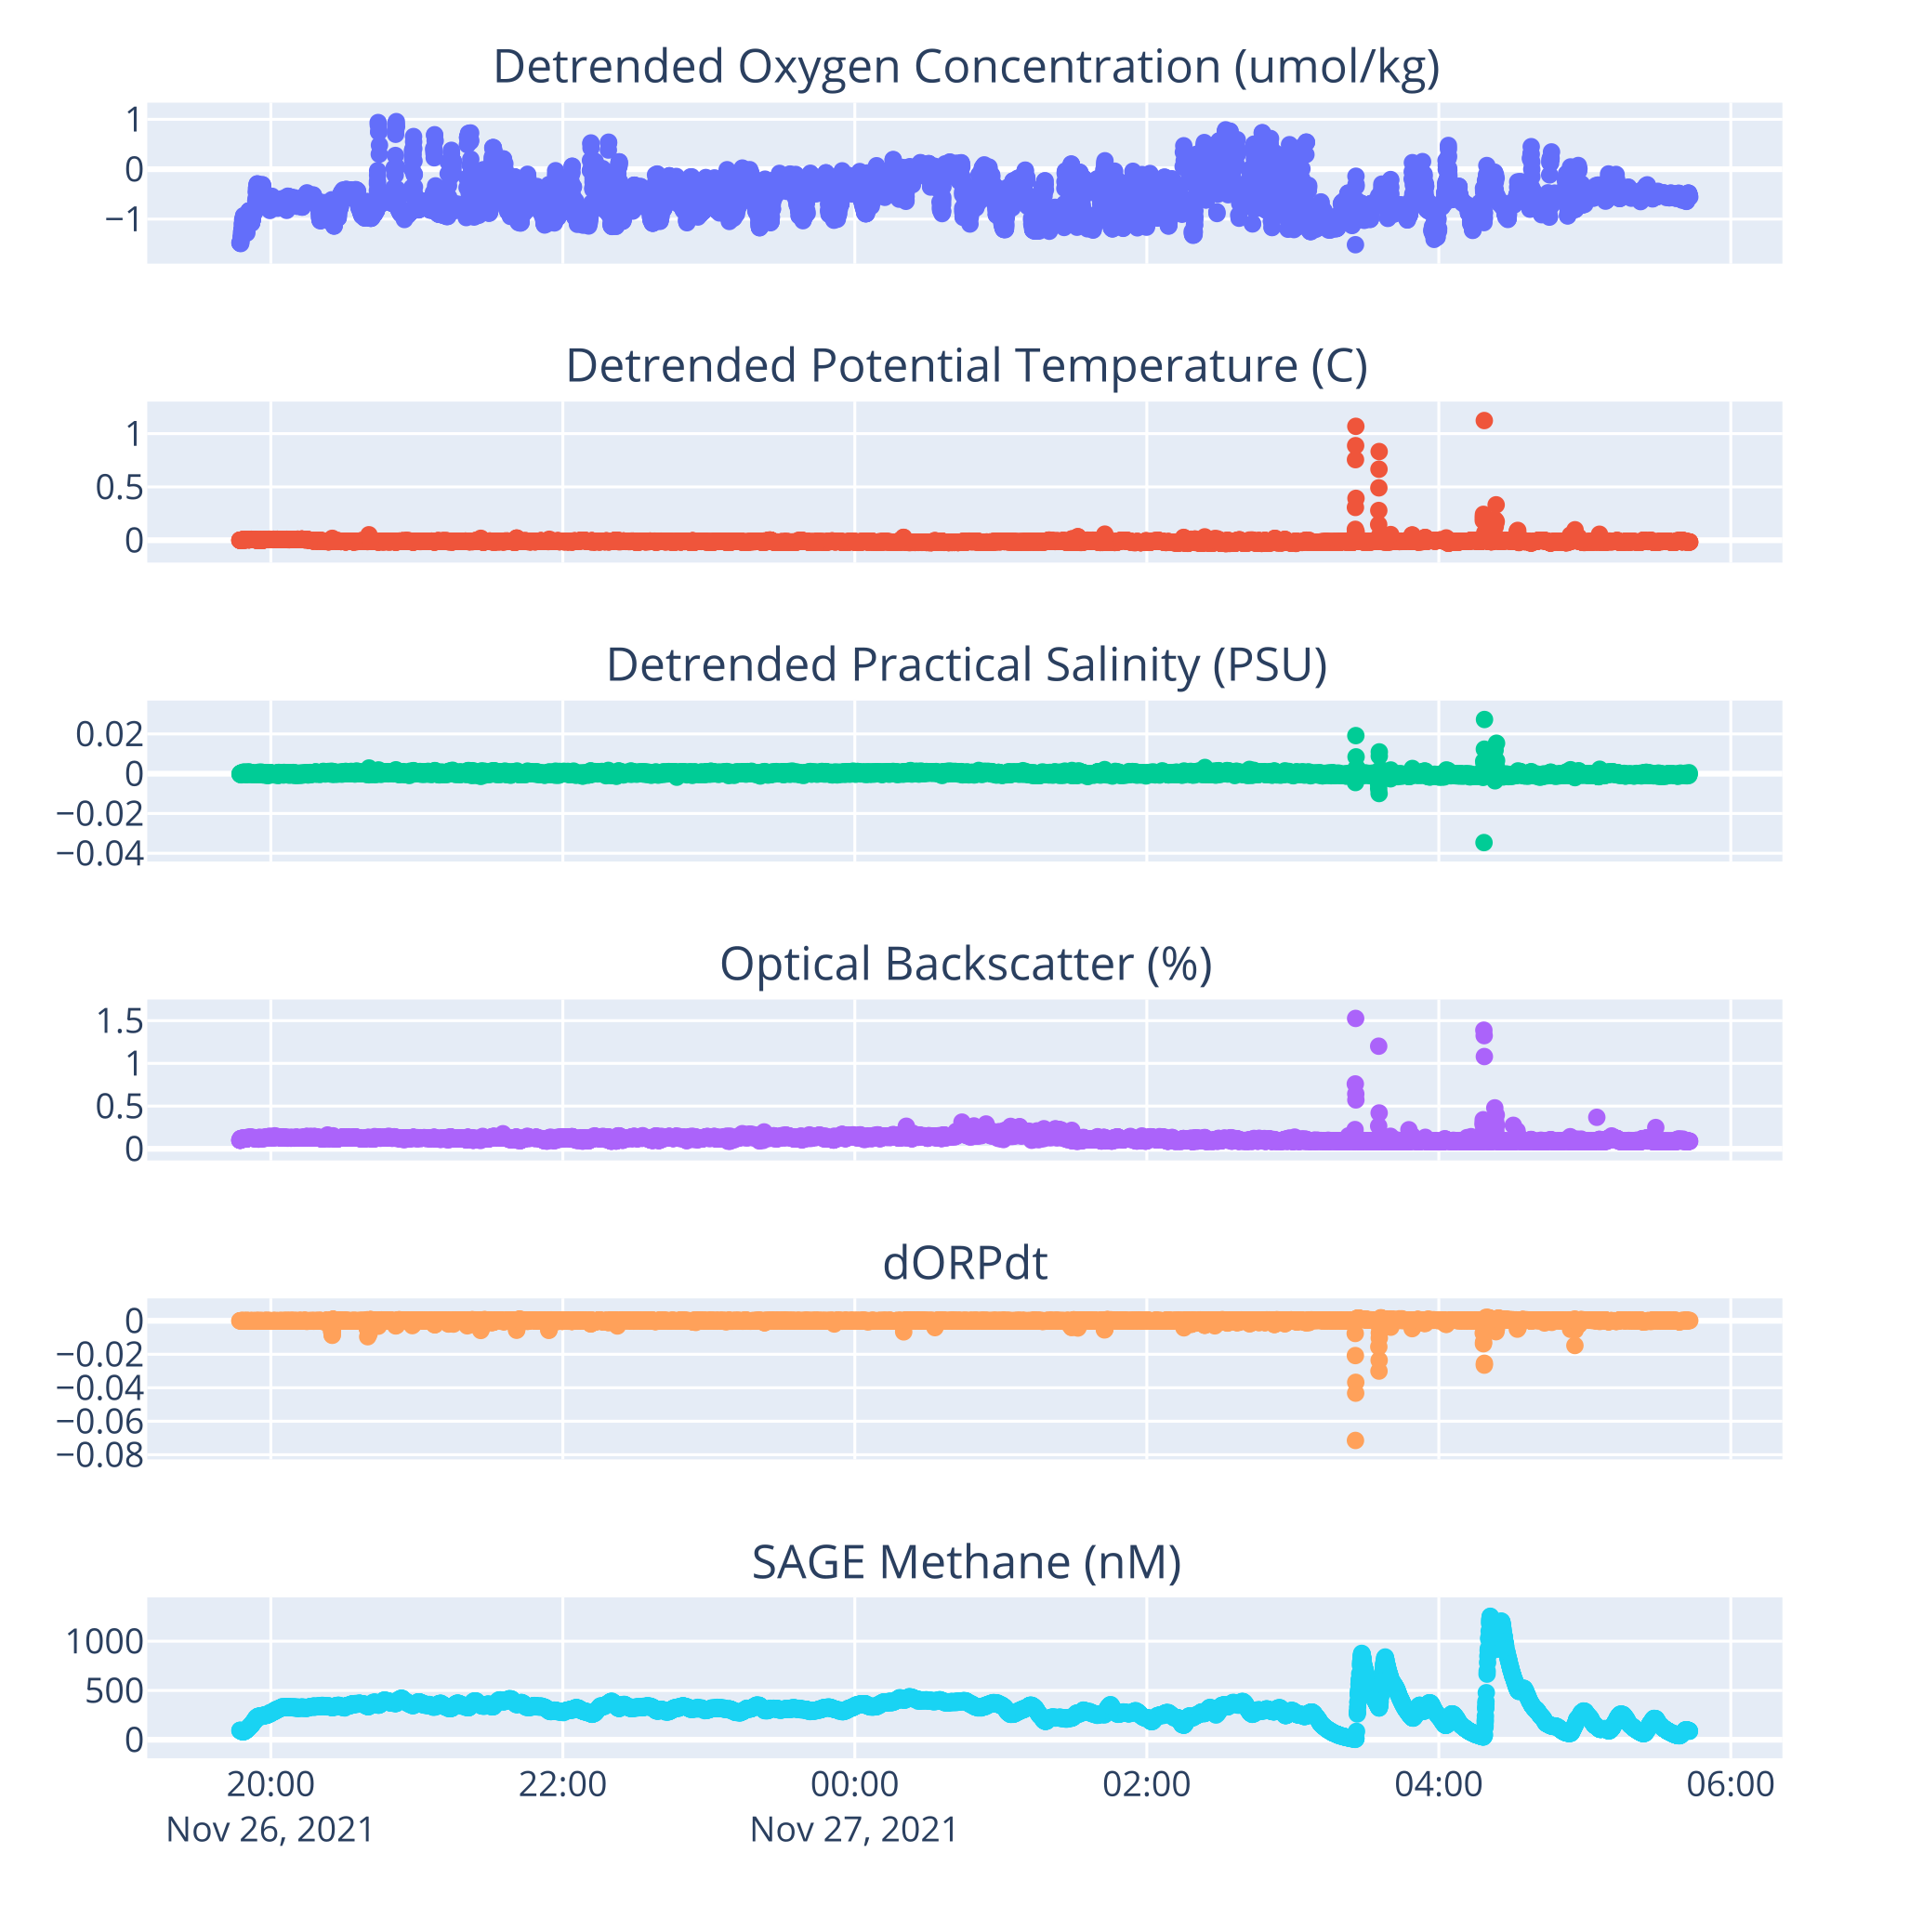
\includegraphics[width=0.45\columnwidth]{figures/binary_example_time.png}
    \hspace{.1in}
    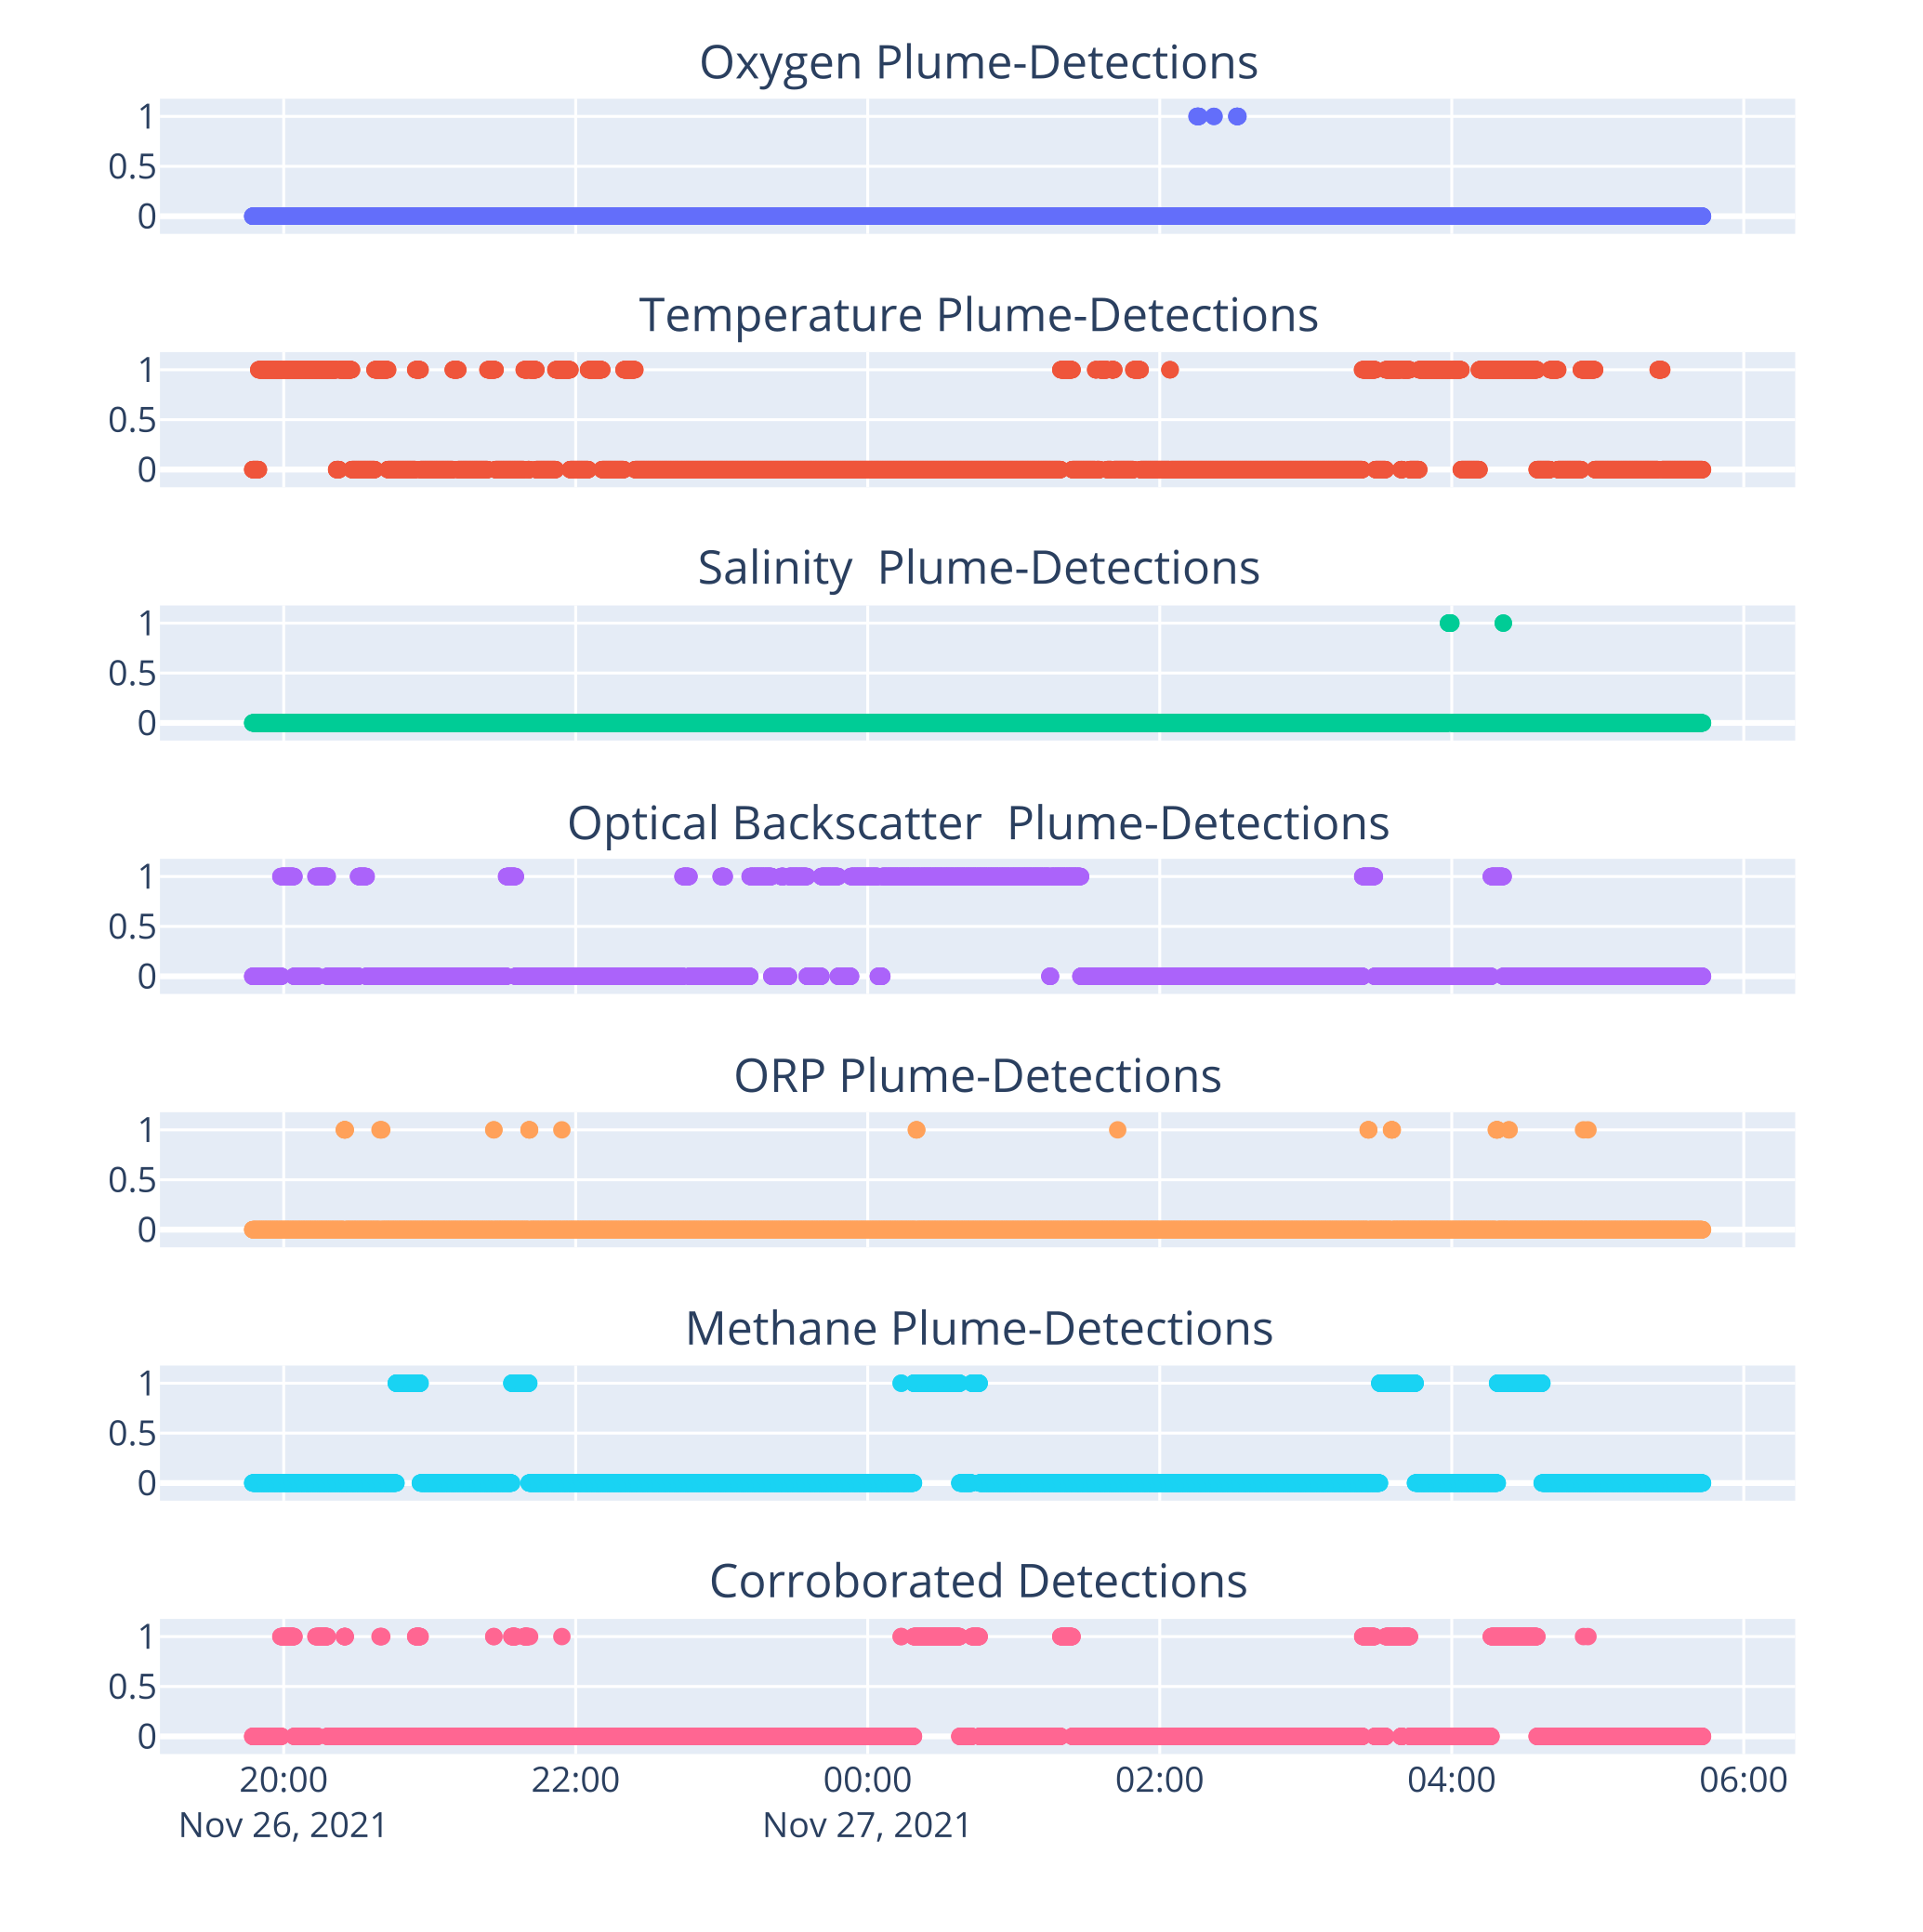
\includegraphics[width=0.45\columnwidth]{figures/binary_example_detections.png}
    \caption[Example time series (left) and associated detections (right) over the AUV \Sentry sensor suite.]{\textbf{Example time series (left) and associated detections (right) over the AUV \Sentry sensor suite.} Oxygen, temperature, and salinity measurements are detrended using a linear transformation fit to depth vs. value plots. The time series demonstrates two types of plume detections. The first are ``obvious detections'' in which most sensors register strong anomalies (this happened twice toward the end of the deployment) and are most strongly associated with buoyant-stem derived fluids. The second are ``persistent-plume detections'' in which the robot traverses through water that is slightly more turbid, warm, or chemical-rich than background water over potentially long horizons (this happened early in the deployment and in the middle). Such detections are most strongly associated with neutrally-buoyant layers. The conservative corroboration detector successfully identifies both forms of plume expressions.}
    \label{fig:detection_example}
\end{figure}

% This approach for processing complex sensor observations into binary plume detections was initially developed by \autocite{jakuba2007stochastic}; our method is an adaptation of the process using recommendations in this previous work and in consultation with the science team we were directly collaborating with for this study. 
The result of our sensor model is to convert multiple, time-stamped sensor observations $s_{t, i} \in \R, \, i = 1, \dots, S$ to a time-stamped binary plume-detection $z_{p, t} \in \{0, 1\}$. These binary plume detections are then used to update \PHUMES and plan robot trajectories with \PHORTEX, as described in \cref{chap:phortex}. The accuracy of this sensor model is difficult to characterize, as there is no available ground truth in a field setting by which to verify the assigned classifications. Qualitatively, the classifications were reviewed by the science team and verified for their alignment with expert opinions on which label to assign.


%%%%%%%%%%%%%%%%%%%
% External Sensing 
%%%%%%%%%%%%%%%%%%
\subsection{Opportunistic Sensing Equipment}
\label{sec:external_current}
Observations from opportunistic external sensors, summarized in \cref{tab:ext_sensors} and visualized in \cref{fig:ext_sensors}, were incorporated into the initial conditions, temporal functions, and seawater properties that define the analytical model in \PHUMES. \PHUMES uses an idealized model of buoyant plume rise under crossflow, the initial conditions of which are the characteristics of the hydrothermal fluids at a vent source. In \PHUMES, these characteristics, represented as $\x_p$, are inference targets. Upon initialization of \PHUMES a uniform prior can be placed over each element of $\x_p$: vent area, fluid velocity at the vent, fluid temperature, fluid salinity, horizontal mixing, and vertical mixing. The bounds on these priors could be informed by previous work or experience by the science team at a a given site, consensus in the literature on physically realistic setpoints, or from \emph{in situ} observations of opportunity during other field operations.

Here, we leveraged access to ROV \emph{JASON} to set prior bounds on vent area and vent fluid exit velocity, and used direct measurements to fix fluid temperature and salinity. \emph{JASON} carries a camera system and temperature wand. Vent area and vent fluid velocity are approximated with images and video captured by ROV \emph{JASON}. Using a \SI{10}{\centi\meter} spaced set of laser points that \emph{JASON} can toggle on and off \emph{in situ}, the vent area is extrapolated from an estimate of vent diameter from pixel-to-distance conversion in still images. Using this method, an area of approximately \SI{1.7}{\meter\squared} was estimated for a coherent cluster of many venting orifices, and used to center a uniform distribution over vent area to be updated with \PHUMES. Vent exit velocity was estimated by applying particle imaging velocimetry (PIV)\autocite{zhang2019time} to 4K video of the turbid fluids at the vent. PIV methods track turbulent parcels that have high cross-correlation values between frames of a video. By tracking many parcels over several frames, PIV yields a vector field of velocity estimates that can be averaged to establish a mean estimate for a region. Using \verb|PIVLab|, an open-source \verb|MATLAB| library, we estimated a fluid exit velocity of \SI{0.7}{\meter\per\second}, and similarly use this as the center of a uniform prior placed on exit velocity for \PHUMES to update. Measuring temperature with an ROV is precise, and so we directly use the observation of temperature by \emph{JASON}, \SI{340}{\celsius}, as the initial condition for vent fluid temperature in the \PHUMES model trained with at-sea data. 

\begin{table}[h!]
    \centering
    \begin{tabular}{c|c|c|c}
        Platform & Instrument & Data Product & \PHUMES Incorporation \\
        \hline
        ROV & Camera & Vent Area & Prior over vent area \\
        ROV & Camera & Fluid Exit Velocity & Prior over fluid exit velocity \\
        ROV & Temperature wand & Vent Temperature  & Temperature initial condition \\
        Rosette & CTD probe & Basin Stratification & Reference for buoyancy model \\
        Tiltmeter & Accelerometer & Crossflow & Trained GP for forecasting \\
    \end{tabular}
    \caption{\textbf{Summary of auxiliary data.} External equipment and opportunistic data available from other operations during the field expedition that was used to inform the \PHUMES model within \PHORTEX used for at-sea trials.}
    \label{tab:ext_sensors}
\end{table}

In addition to \emph{JASON}, vertical profiles from a rosette of ambient seawater background salinity and temperature were available. Within \PHUMES, a reference stratification curve is used to compute depth-dependent buoyancy force. To set this curve in previous simulation work (\cref{chap:phortex}), we used a widely accepted set of equations of state for Pacific temperature, Pacific salinity, and density as described in~\cite{speer1987model}. As stratification plays a nontrivial role in the ultimate expected rise height of a plume, access to a better model of stratification for a test site will improve prediction quality. At sea, these equations can be directly approximated for a given water mass using data gathered during standard vertical transects with a rosette. To compute these curves, which will be fixed for the purposes of \PHUMES, a single rosette profile of temperature and salinity collected early in the expedition were fit by vanilla Gaussian Process (GP) models with radial-basis function (RBF) kernels using \verb|GPytorch| (100 iterations, learning rate 0.1), and the trained mean function of those models was used within \PHUMES.

Finally, we learn the crossflow transition function $T_c$. Critically there was no sensor on \Sentry during our expedition that could be used to measure the \emph{in situ} current magnitude and heading\footnote{It is somewhat normal for such a sensor to exist. Acoustic Doppler Current Profilers (ADCPs) are common sensors used with a Doppler velocity logger (DVL) for AUV navigation. Lack of ADCP for the purposes of water column measurements on this cruise was largely a consequence of ongoing vehicle improvement and a yet untested system. For the sake of this work, we can assume that \emph{in situ} point observations of crossflow is generally possible.}. While it may be possible to estimate $T_c$ solely from the binary observations of the plume, access to an external bottom-mounted tiltmeter on the seafloor during this expedition significantly relieved the burden of this inference process. A tiltmeter is an instrument that is fixed to the seafloor on one end, and is allowed to tilt under the effects of crossflow. Using ROV \emph{JASON}, two tiltmeters were intermittently deployed for several days during the cruise, and approximately three days of data were used to compute crossflow magnitude and heading. We observed a maximum crossflow magnitude of approximately \SI{0.13}{\meter\per\second}, with heading sweeping between north-northwest to southwest. Both magnitude and heading appeared to be semi-cyclic, following a time-lagged pattern established by tidal charts produced by Centro de Investigaci\'on Cient\'ifica y de Educaci\'on Superior de Ensenada (CISESE) for the time period of the expedition\footnote{Charts available from: \url{www.predmar.cicese.mx/calendarios}}. Time-varying current magnitudes between 0.1-\SI{0.5}{\meter\per\second} sweeping from the northwest to southwest were previously reported in \autocite{scholz2019shelf}, corroborating our observations. We trained a GP with RBF kernel for each of current magnitude and heading over hour of the day using \verb|GPytorch| (magnitude model: 100 training iterations, learning rate 0.5; heading model: 200 training iterations, learning rate 0.1), and used the entire trained GP within the sampling framework for \PHUMES to generate forecasts, allowing us to account for uncertainty in the crossflow functions. 

\begin{figure}[h!]
    \centering
    \includegraphics[width=1\columnwidth]{figures/external_sensors.png}
    \caption[Auxiliary data products used in \PHUMES.]{\textbf{Auxiliary data products used in \PHUMES.} External equipment (ROV \emph{JASON}, tiltmeter, and rosette) provided opportunistic data products during the field expedition that were incorporated into \PHUMES. The ROV \emph{JASON} was used to determine prior estimates for the plume source parameters. The rosette collected vertical temperature and salinity profiles which are used to compute stratification in the basin. A GP is trained over each of the temperature and salinity data, and the mean is visualized over the data in the lower right panel. The tiltmeter records data of current magnitude and heading; a GP was trained over both functions and is visualized in the lower left panel. Heading is reported in compass-rose orientation.}
    \label{fig:ext_sensors}
\end{figure}


\subsection{At Sea Operations}
\PHORTEX was used to enable deployment-by-deployment autonomy during field operations with AUV \emph{Sentry} that fit within the typical workflow of operations at sea (\cref{fig:at_sea_ops}). Functionally, the trajectories planned with \PHORTEX were provided to the \Sentry engineering team for extensive safety validation prior to each deployment. If approved by the \Sentry team, the chief scientist, and any other stakeholders, the trajectories were downloaded into the \Sentry mission planning software as static waypoints. This confirmation process required a lead time of approximately 6 hrs before a scheduled deployment, and 12-18 hrs were available between deployments to mechanically service \Sentry and recharge batteries. The ability of \PHORTEX to produce viable trajectories from data within the first 6 hrs that \Sentry was on-deck following a recovery was critical for keeping this strict timeline. The flexibility in the \PHUMES chaining procedure (number of samples to simulate) and the \PHORTEX optimizer (optimization steps for a trajectory), allow us to scale planning computation time within whatever window is available. Given the long lead time between trajectory design and \Sentry deployment, there were many opportunities for the time of a deployment to change due to e.g., developments in weather, or other science/technology priorities. To be robust to these changes, we provided deployment plans that started several hours before and lasted several hours after a given deployment window, and the \Sentry team could snip the irrelevant links from the chain once a deployment time was known with certainty.

\begin{figure}[h!]
    \centering
    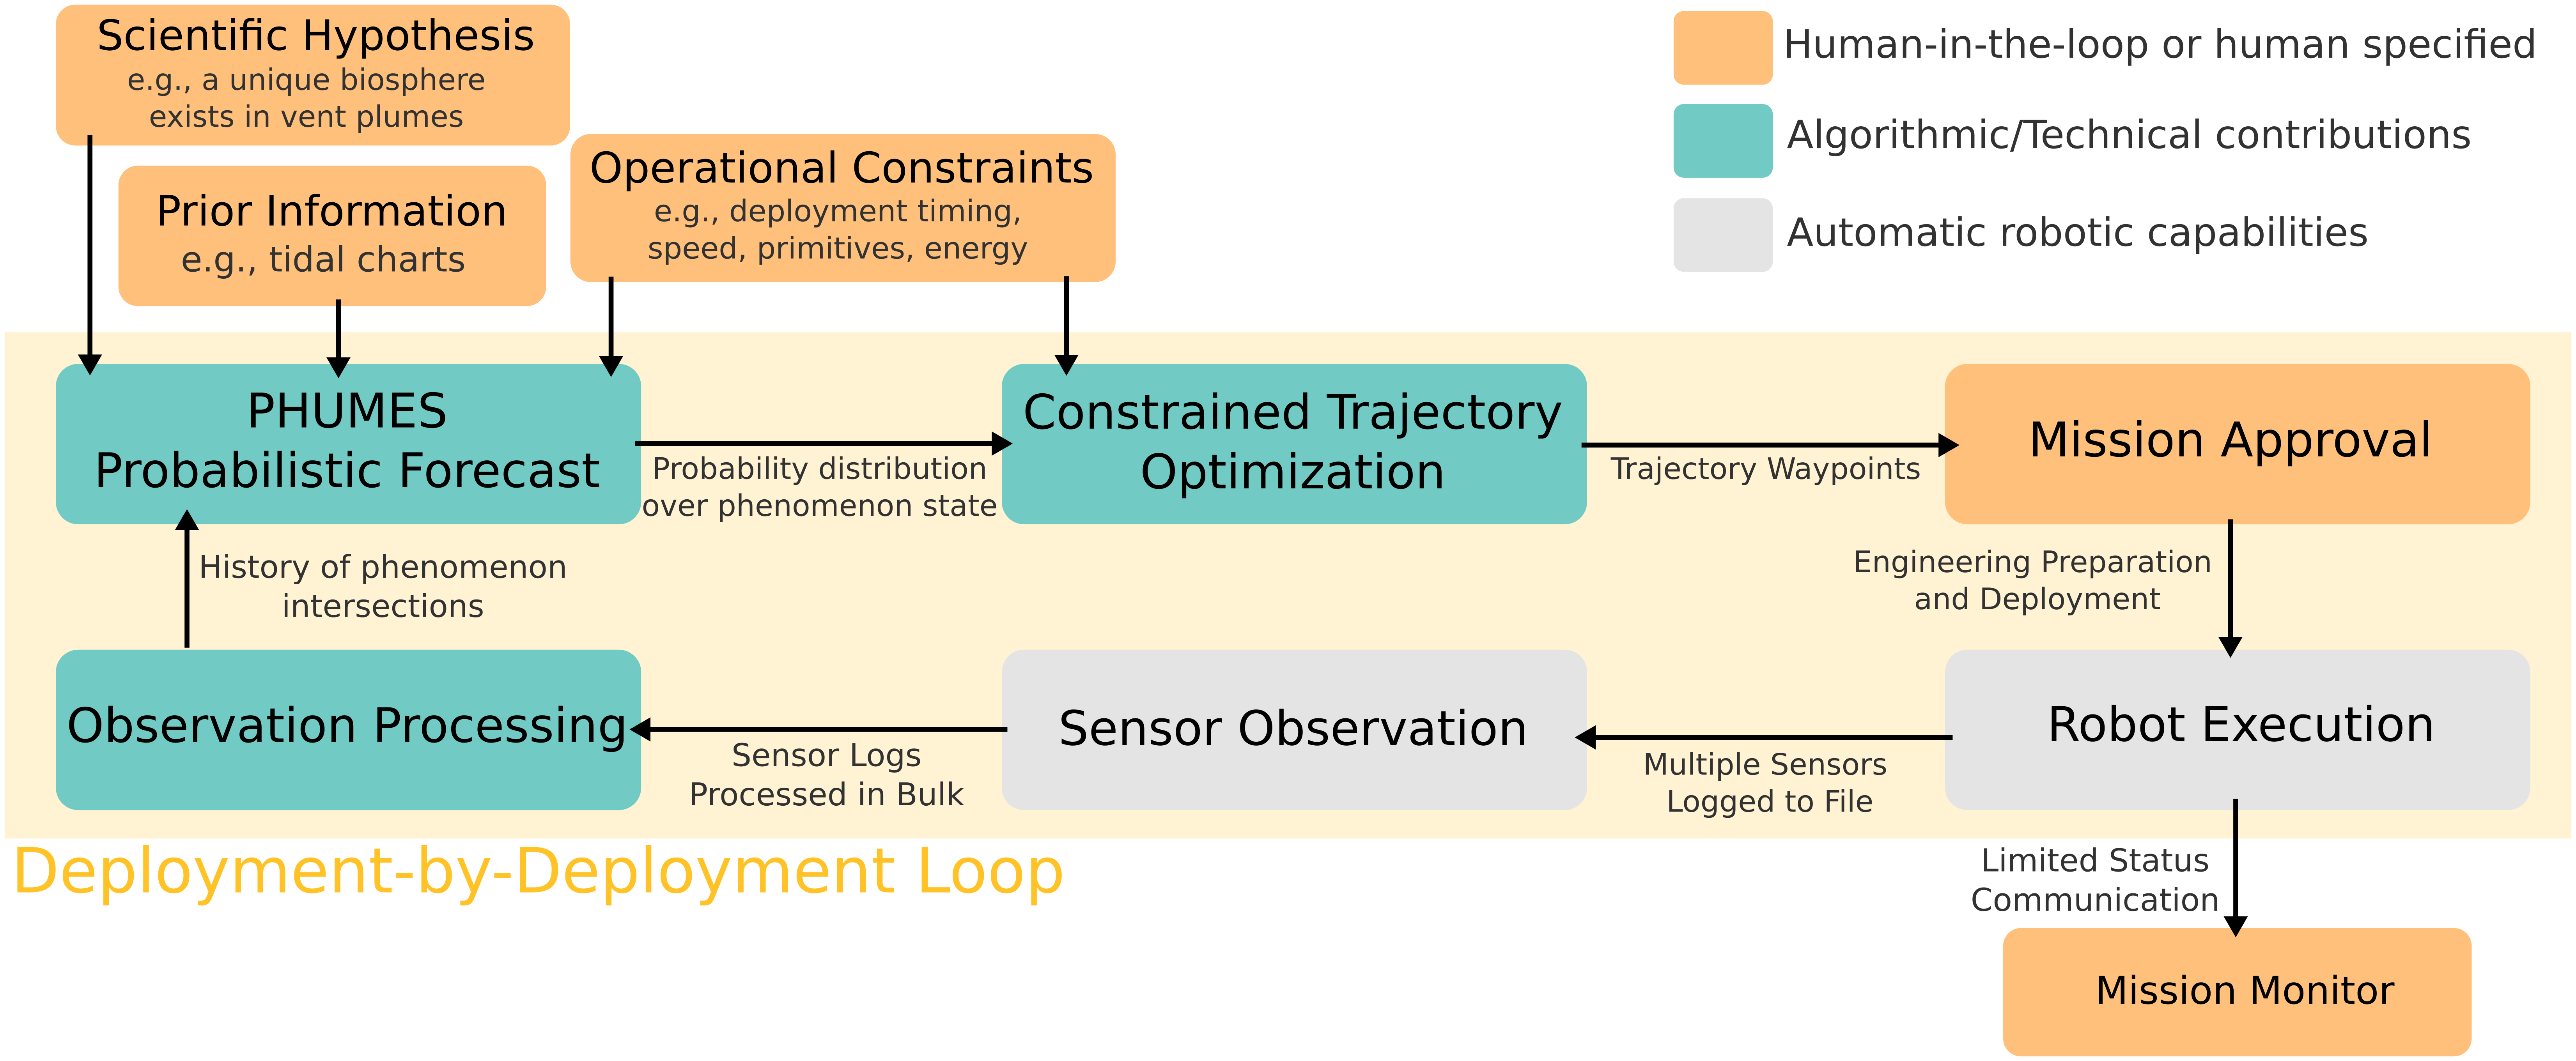
\includegraphics[width=1.0\columnwidth]{figures/deployment_loop.png}
    \caption[The operational implementation of \PHORTEX at sea.]{\textbf{The operational implementation of \PHORTEX at sea.} Integration of scientific knowledge, prior information, auxiliary sensor information, and operational constraints was done at the initialization of the \PHORTEX deployment-by-deployment loop. Every trajectory generated by \PHORTEX was checked by AUV \Sentry engineers and the science team before execution. \Sentry status was monitored with an external acoustic tracking system that monitored vehicle location, power, and performance while in acoustic range of the ship. Upon returning to deck, all science sensor observations were downloaded in bulk from the vehicle, and then ingested via our \PHORTEX system to plan a new dive.}
    \label{fig:at_sea_ops}
\end{figure}

When \Sentry completed a dive, it was brought onto deck and within the first hour of being returned, data products from the vehicle were available over the \Sentry local network. Separate files for each sensor were downloaded, processed in the way described in \cref{sec:field_sensor_models}, and used to immediately begin a \PHUMES update. In general, waiting until the end of a dive before anything is known about what the science sensors ``saw'' while underway is typical. The \Sentry team usually provides summary reports about the performance of the science sensors several hours after a dive. This is in sharp contrast with navigational data reporting, which is often updated live on visual monitors while \Sentry is underway and within acoustic communication range of a ship. Since on-the-fly planning changes are generally not allowable (unless to fix a drifting \Sentry state estimation), and communication latency is approximately 0.02 Hz, there is not generally support for visualizing the science data while \Sentry is surveying. For this cruise, we requested that science data be relayed to the ship when possible, and created a live-updating visualization of the key science sensors for hydrothermal mapping. While it did not play a critical role in the operations we conducted for \PHUMES and \PHORTEX, there was considerable excitement and interest in looking at this data. Anecdotally, it was clear that even with significantly sub-sampled data being reported by \Sentry, hydrothermally driven anomalies could be spotted in the data, potentially making a future for an online version of \PHUMES within reach to support ongoing ship-based activities while \Sentry is underway. 


\section{Description of the Autonomy Field Work}
Testing of \PHORTEX during field trials to the Guaymas Basin, described in \cref{sec:guaymas_description}, largely took place at the Northern Ridge site, targeting a particular venting chimney at decimal coordinates (27.412645N, 111.386915W) located at a depth of approximately \SI{1850}{\meter} (\cref{fig:autonomy_site}). 

\begin{figure}[h!]
    \centering
    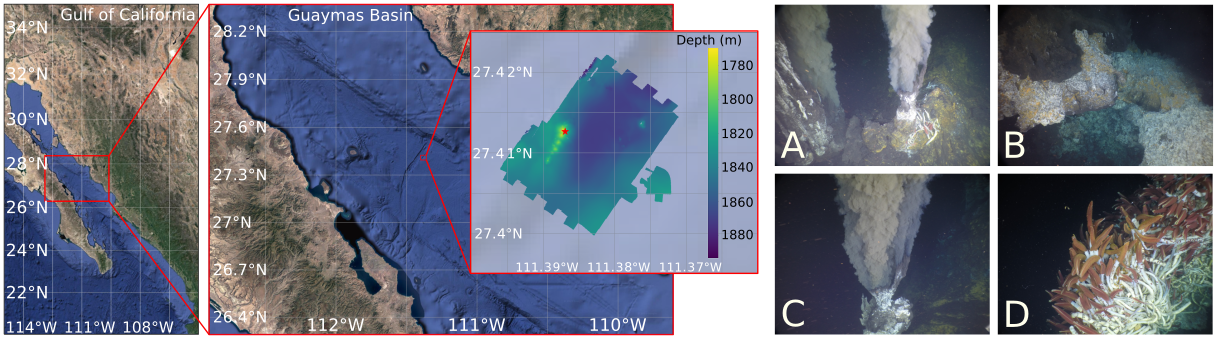
\includegraphics[width=\columnwidth]{figures/site_summary.png}
    \caption[Study sit in the Guaymas Basin, Gulf of California]{\textbf{Study site in the Guaymas Basin, Gulf of California.} The inset map is bathymetric data collected by AUV \Sentry during this expedition and shows the approximately \SI{600}{\meter} long ridge in yellow. The red star marks the chimney that was of particular study in this article. Pictures A-D show imagery from the ridge and chimney site. A-C show various forms of plume-producing vents located at the chimney and D shows an example of the macrofauna covering the structures along the ridge.}
    \label{fig:autonomy_site}
\end{figure}

\subsection{Dives}
\label{sec:field_dives}
Four deployments of AUV \Sentry were available to study the northern chimney site. These deployments represent a planning spectrum, from fully human-designed surveys to fully \PHORTEX designed. We label the four deployments as follows:
\begin{itemize}
    \item \textbf{Dive H-Multi}: human designed, multi-task survey. This was the first deployment of \Sentry and the survey was designed to both attempt to find plume fluids and to bathymetrically map the local basin area (the map of which would be used as part of the safety check protocol for future deployments). This dive is representative of a standard nested strategy, in which progressively more targeted (finer resolution) surveys are used to study areas of interest. The dive was designed by a human expert who only had access to the approximate location of the target vent. The deployment lasted 21.3 hrs and collected 76,604 observations total.
    \item \textbf{Dive H-Plume}: human designed, plume-charting survey. This was the second deployment of \Sentry and the survey was hand-designed by the science party onboard the vessel to find and sample plume fluids. The science party had access to the performance of \Sentry in Dive H-Multi. The strategy was to sweep the basin above areas with known hydrothermal vents, and fly out into the basin in the direction that the plume fluids would be expected to advect. The deployment lasted 21 hrs and collected 75,430 observations total.
    \item \textbf{Dive HP-Plume}: hybrid human and \PHORTEX plume-charting survey. This was the third deployment of \Sentry and the survey consisted of trajectories designed by \PHORTEX trained by observations collected only in Dive H-Multi. Two of the trajectory primitives designed by \PHORTEX were replaced by ``naive'' lawnmowers placed over the known vent at two different times in the deployment. The deployment lasted 22.2 hrs and collected 79,792 observations total. Of these, 8.2 hrs and 29,438 observations were collected via the naive strategy.
    \item \textbf{Dive P-Plume}: \PHORTEX plume-charting survey. This was the fourth and last deployment of \Sentry. The survey was fully designed by \PHORTEX using observations only from Dive H-Multi, several days prior to this dive. The deployment lasted 9.9 hrs and collected 35,755 observations total. This deployment is notably much shorter than the other deployments due to increasing time constraints as the expedition was coming to a close. This deployment also used \Sentry in a ``depth-hold'' mode: whereas in all other dives \Sentry's depth followed the basin terrain, in this experiment the robot held an absolute depth.
\end{itemize}

\subsection{Evaluation of Field Data}
\label{sec:field_eval_metrics}
Using the metrics introduced in \cref{sec:eval_metrics}, we evaluate each of the four dives executed at sea to chart the space-time dynamics of a real hydrothermal plume. Each dive took place at different times in the tidal cycle, on different days, and often at different altitudes in the water column, and thus the total plume samples available to collect during each dive is variable. With this in mind, we present and evaluate each dive quantitatively, and additionally qualitatively examine each as a case study for how different sampling paradigms perform in the real-world. There is no ground-truth available for the deep sea plume-charting problem; we evaluate each \Sentry dive assuming that the binary detections produced by the method in \cref{sec:field_sensor_models} are honest representations of the presence or absence of hydrothermally derived fluids in the basin. 

\section{Performance of \PHORTEX}
\label{sec:phortex_performance}
The results of the field deployment presented in \cref{tab:field_results} and visualized in \cref{fig:field_results} demonstrate that \PHORTEX performs comparably to science expert-designed trajectories in the proportion of samples that are collected during dives, and importantly improves upon the spatial utilization (increasing both the range of the most distal plume detection and effectively utilizing of the entire explored range). This is most evident in the HP-Plume dive, in which the human designed portion is a lawnmower trajectory placed ``on top'' of the vent; the \PHORTEX-designed trajectory collects samples over twice as far from the plume source. Absolute temporal utilization is similar to human surveys; however the distribution of detections within the temporal utilization windows is improved --- for human surveys, detections tend to be ``bunched'' to either the first half (as in H-Plume) or second half (as in H-Multi). We see this most sharply in HP-Plume, in which 90\% of positive detections collected by the human-designed survey occurred only in the second of the two lawnmowers, from hours 20-22. In contrast, \PHORTEX designed trajectories collected detections more uniformly over the entire \PHORTEX portion of the HP-Plume dive. \cref{fig:field_results} shows the qualitative structure of each dive and showcases the diversity in the resulting datasets.

\begin{table}[h!]
    \centering
    \begin{tabular}{c|c|c|c|c|c}
        Dive & Duration & Total Obs. & In-Plume & Spatial Util. & Temporal Util.  \\
        \hline
        H-Multi & 21.3 hrs & 76,604 & 22.3\% & \SI{300}{\meter} (19\%) & 9-17,20-21 (52\%) \\
        \hline
        H-Plume & 21 hrs & 75,430 & 10.9\% & \SI{900}{\meter} (64\%) & 2,5-8,10-11,15-16 (43\%) \\
        \hline
        HP-Plume & 22.2 hrs & 79,792 & 41.8\% & \SI{600}{\meter} (100\%) & 1-3,5,7,11-22 (77\%) \\
        (H) & 8.2 hrs & 29,438 & 42.3\% & \SI{250}{\meter} (100\%) & 5,20-22 (49\%) \\
        (P) & 14 hrs & 50,354 & 41.5\% & \SI{600}{\meter} (100\%) & 1-3,7,11-19 (93\%)\\
        \hline
        P-Plume & 9.9 hrs & 35,755 & 12.8\% & \SI{450}{\meter} (100\%) & 1,5,8,9 (40\%)
    \end{tabular}
    \caption[Per-dive statistics for field trials of \PHORTEX.]{\textbf{Per-dive statistics for field trials of \PHORTEX.} The spatial utilization is reported as both the most distal plume detection (measured from the plume origin) and the ratio of the most distal plume detection over the farthest distance that the robot traveled from the plume origin. Temporal utilization shows both which hours contain at least 10\% positive plume detection and what fraction of the total deployment duration contained such detections. The deployment HP-Plume is broken further into human designed (H) and \PHORTEX designed (P) portions for direct comparison.}
    \label{tab:field_results}
\end{table}

\begin{figure}[h!]
    \centering
    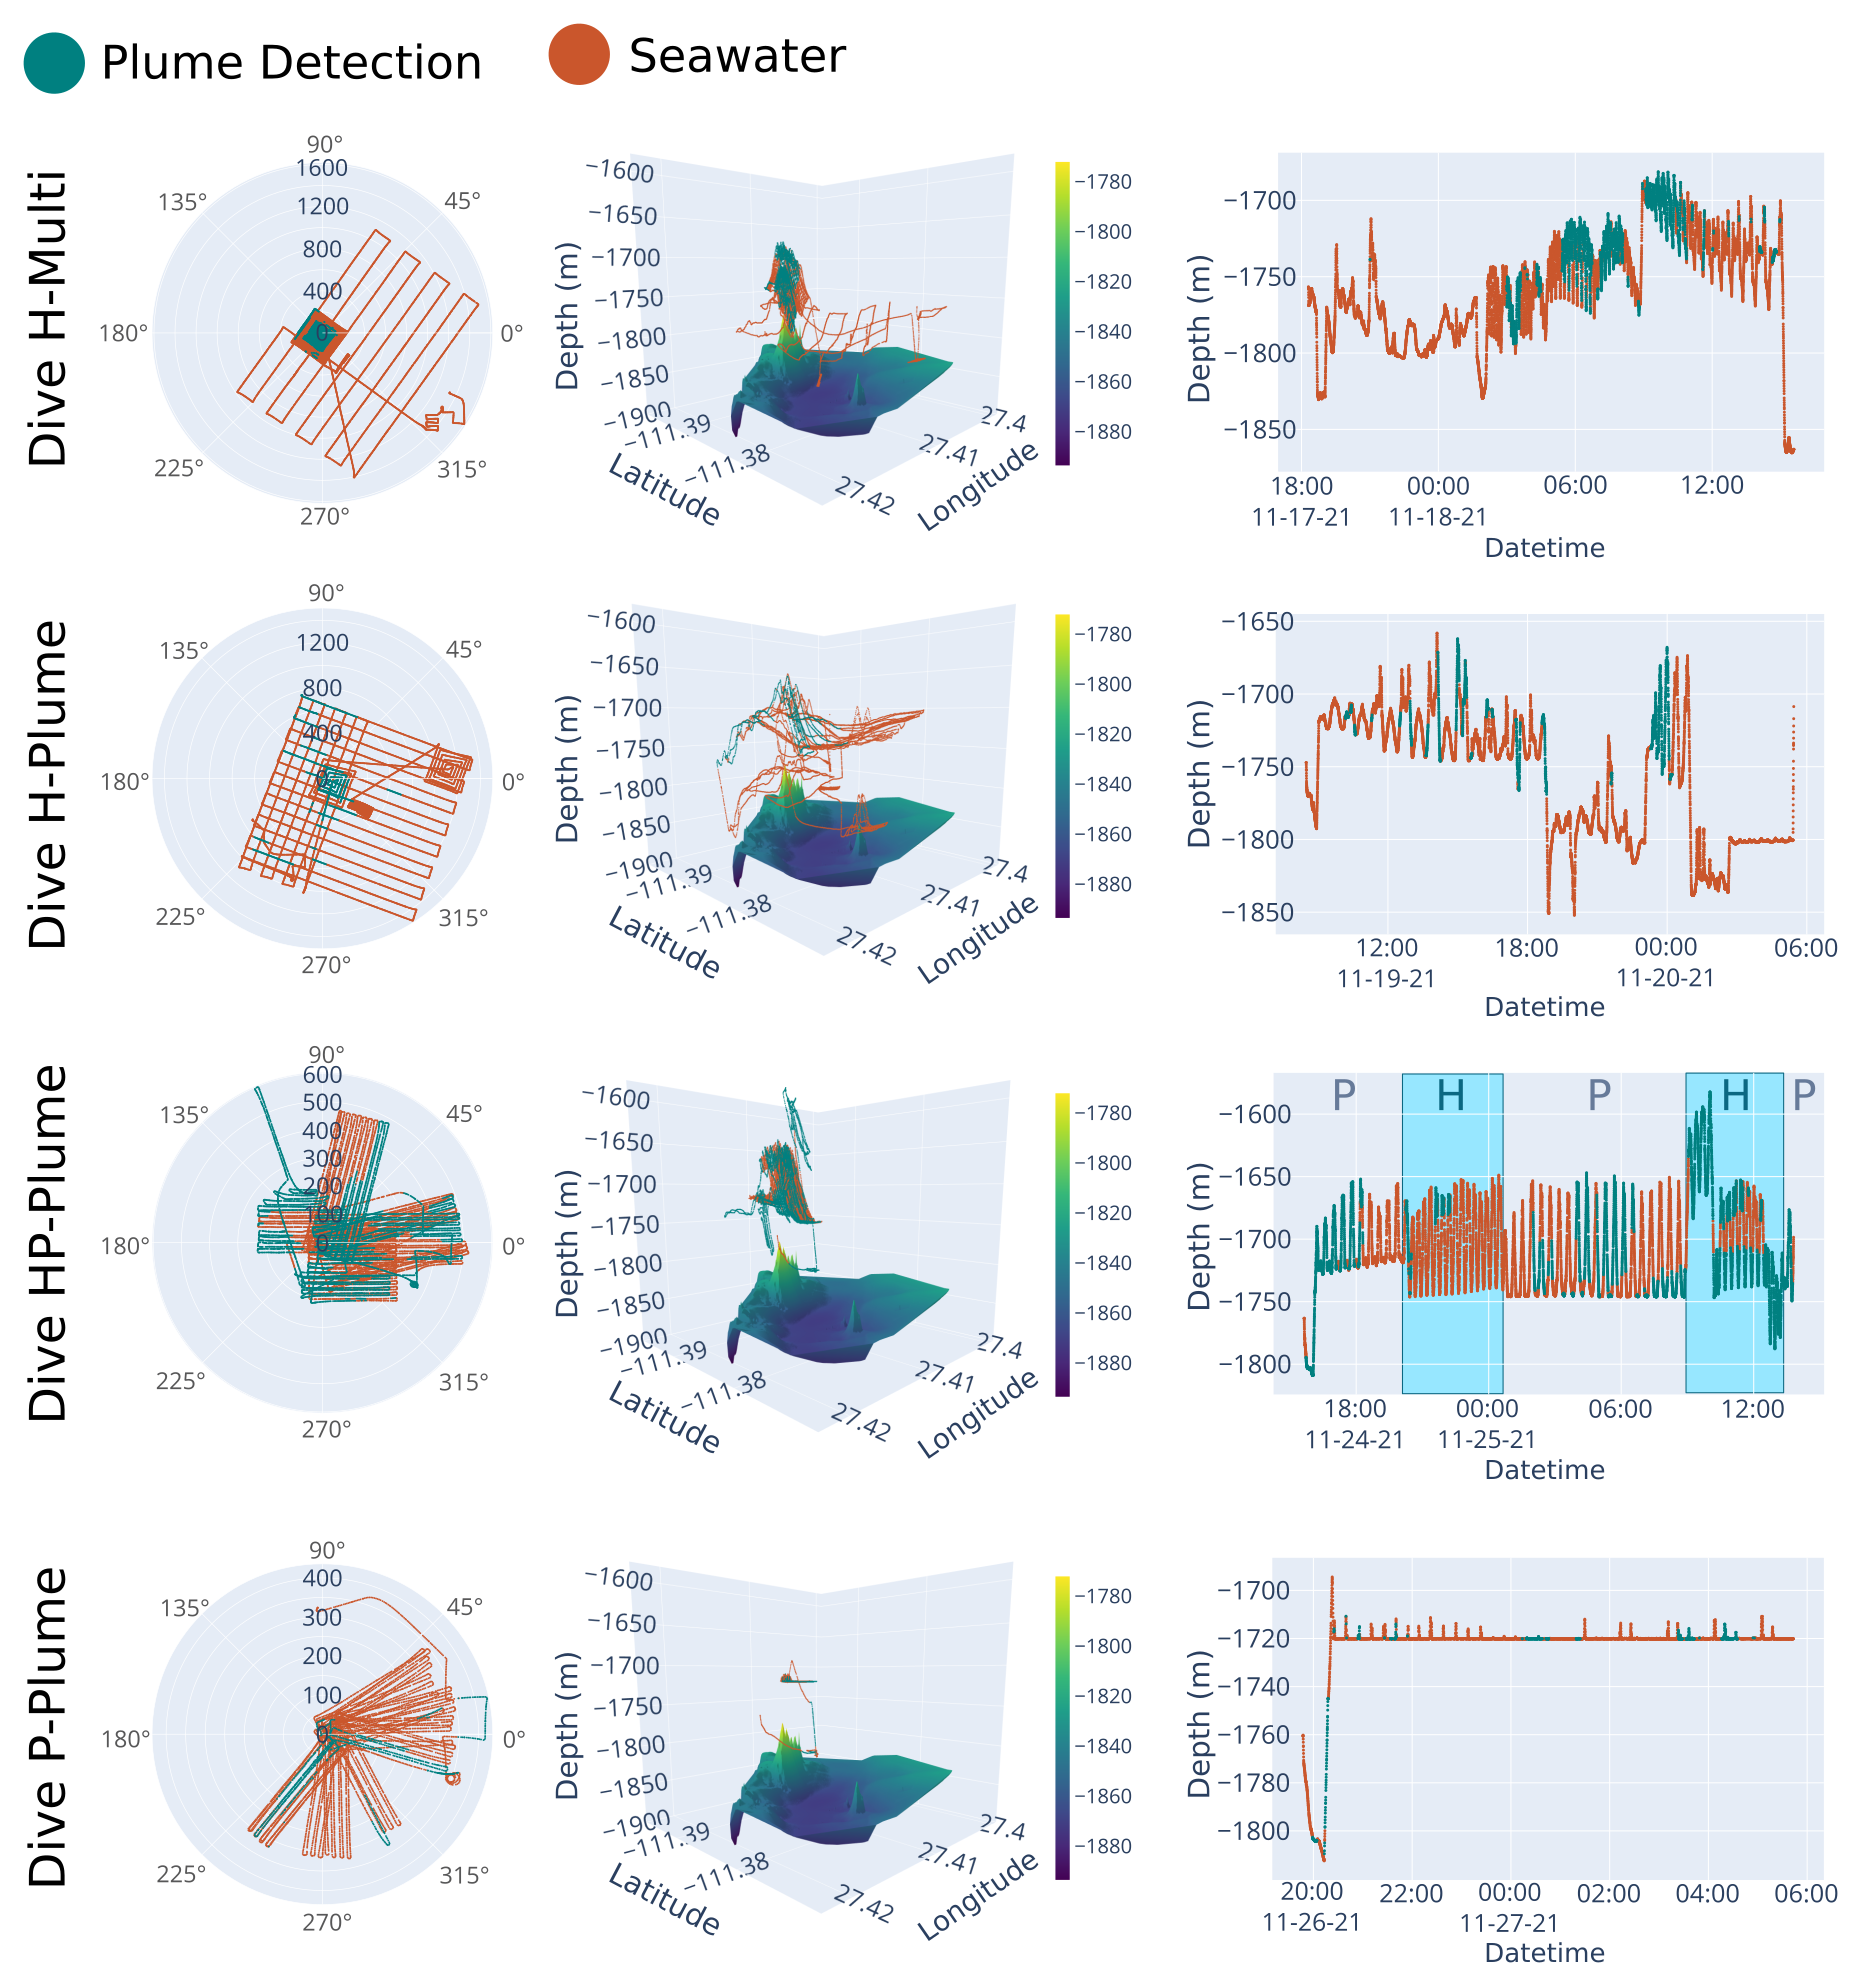
\includegraphics[width=0.85\linewidth]{figures/detections_data.png}
    \caption[The four field dives of AUV \Sentry.]{\textbf{The four field dives of AUV \Sentry.} All data is plotted according to its detection identity (in-plume or seawater). The first column shows a top-view of the dive trajectories in polar coordinates, in which angle and radius is computed relative to the chimney coordinate of the vent of study. In the center column, the 3D path of the vehicle over the rendered bathymetric terrain is provided. All but Dive P-Plume were dives conducted in altitude-hold mode with \Sentry, and so the trajectories show obvious changes in elevation; in contrast Dive P-Plume was held in depth-hold mode, so most observations are gathered within a depth-plane. The final column shows a time series versus depth of the detections collected. In Dive HP-Plume the portions of the dive that were human-designed and \PHORTEX-designed are labeled with H and P, respectively. As can be seen in the Dive HP-Plume time series, the two human-designed trajectories have significantly different performance, despite being in locally similar regions of the spatial domain. }
    \label{fig:field_results}
\end{figure}

In this field deployment, we demonstrate that \PHORTEX is a useful and practical tool for plume-charting. The performance of trajectories designed with \PHORTEX are comparable to those designed by human experts with key improvements in spatial and temporal utilization. It is further worth highlighting that \PHORTEX was trained only on data collected during the first dive, H-Multi, and reasonable performance during P-Plume using week-old training data (slightly improved total number of detections over H-Plume given the same initial information, improved spatial utilization, and more evenly encountered plume detections) emphasizes the long-range forecasting ability of the approach. Practically, the automated nature of \PHORTEX operationally alleviates significant decision-making burden on a science team and the trajectory-design burden on the \Sentry team; the ability to ingest data from external sensors and previous \Sentry missions, and produce trajectories that can be seamlessly ingested by the safety checking system without human intervention is of considerable benefit in the field. Moreover, by virtue of yielding rich context easily interpretable by the science team, the intermediate products of \PHORTEX like \PHUMES forecasts, are useful for other tasks in field operations, such as deploying other instruments or prioritizing instrument deployment order based on temporal changes in the environment. 

% Similarly, \PHORTEX is trained on significantly less data than what the human experts had access to throughout the cruise; this emphasizes the advantage of the model-based, data-aggregation approach in \PHUMES. 

\section{\PHUMES Validation with Basin Observations}
\label{sec:field_phumes}
While there is no external ``ground-truth'' that we can use to evaluate the performance of \PHORTEX, we can compare the \PHUMES model trained on external and binary \Sentry observations with snapshots of the vertical distribution of turbidity near the hydrothermal ridge to get a sense of the explanatory power of the \PHUMES model. After training, \PHUMES estimated the fluid exit velocity from the target chimney to be \SI{0.58}{\meter\per\second}, the vent area to be \SI{0.82}{\meter\squared}, and the vertical and horizontal mixing coefficients to be 0.15 and 0.19, respectively. Simulating these conditions with an initial vent temperature of \SI{340}{\celsius} and salinity of 34.908 PSU under a nominal crossflow of \SI{0.11}{\meter\per\second}, we compare the time-averaged plume height and width with the turbid intrusion that are observed in vertical casts of a shipboard rosette. The rosette was lowered and raised through the water column using a cable and winch on the ship; several vertical transects were collected over the course of the research cruise near the target autonomy site in addition to other sites throughout the basin. In \cref{fig:field_valid} we show two vertical transects, one conducted about \SI{100}{\meter} from a known vent, and one conducted \SI{600}{\meter} from the same vent. We see that within the model regions for predicted plume intrusions in the water column, strong turbid signals are observed in both vertical transects. This is indicative that the learned \PHUMES model is capable of uncovering the structure of the hydrothermal plume and lends confidence that the model is informative for planning sample trajectories that will intersect with plume fluids.

\begin{figure}[h!]
    \centering
    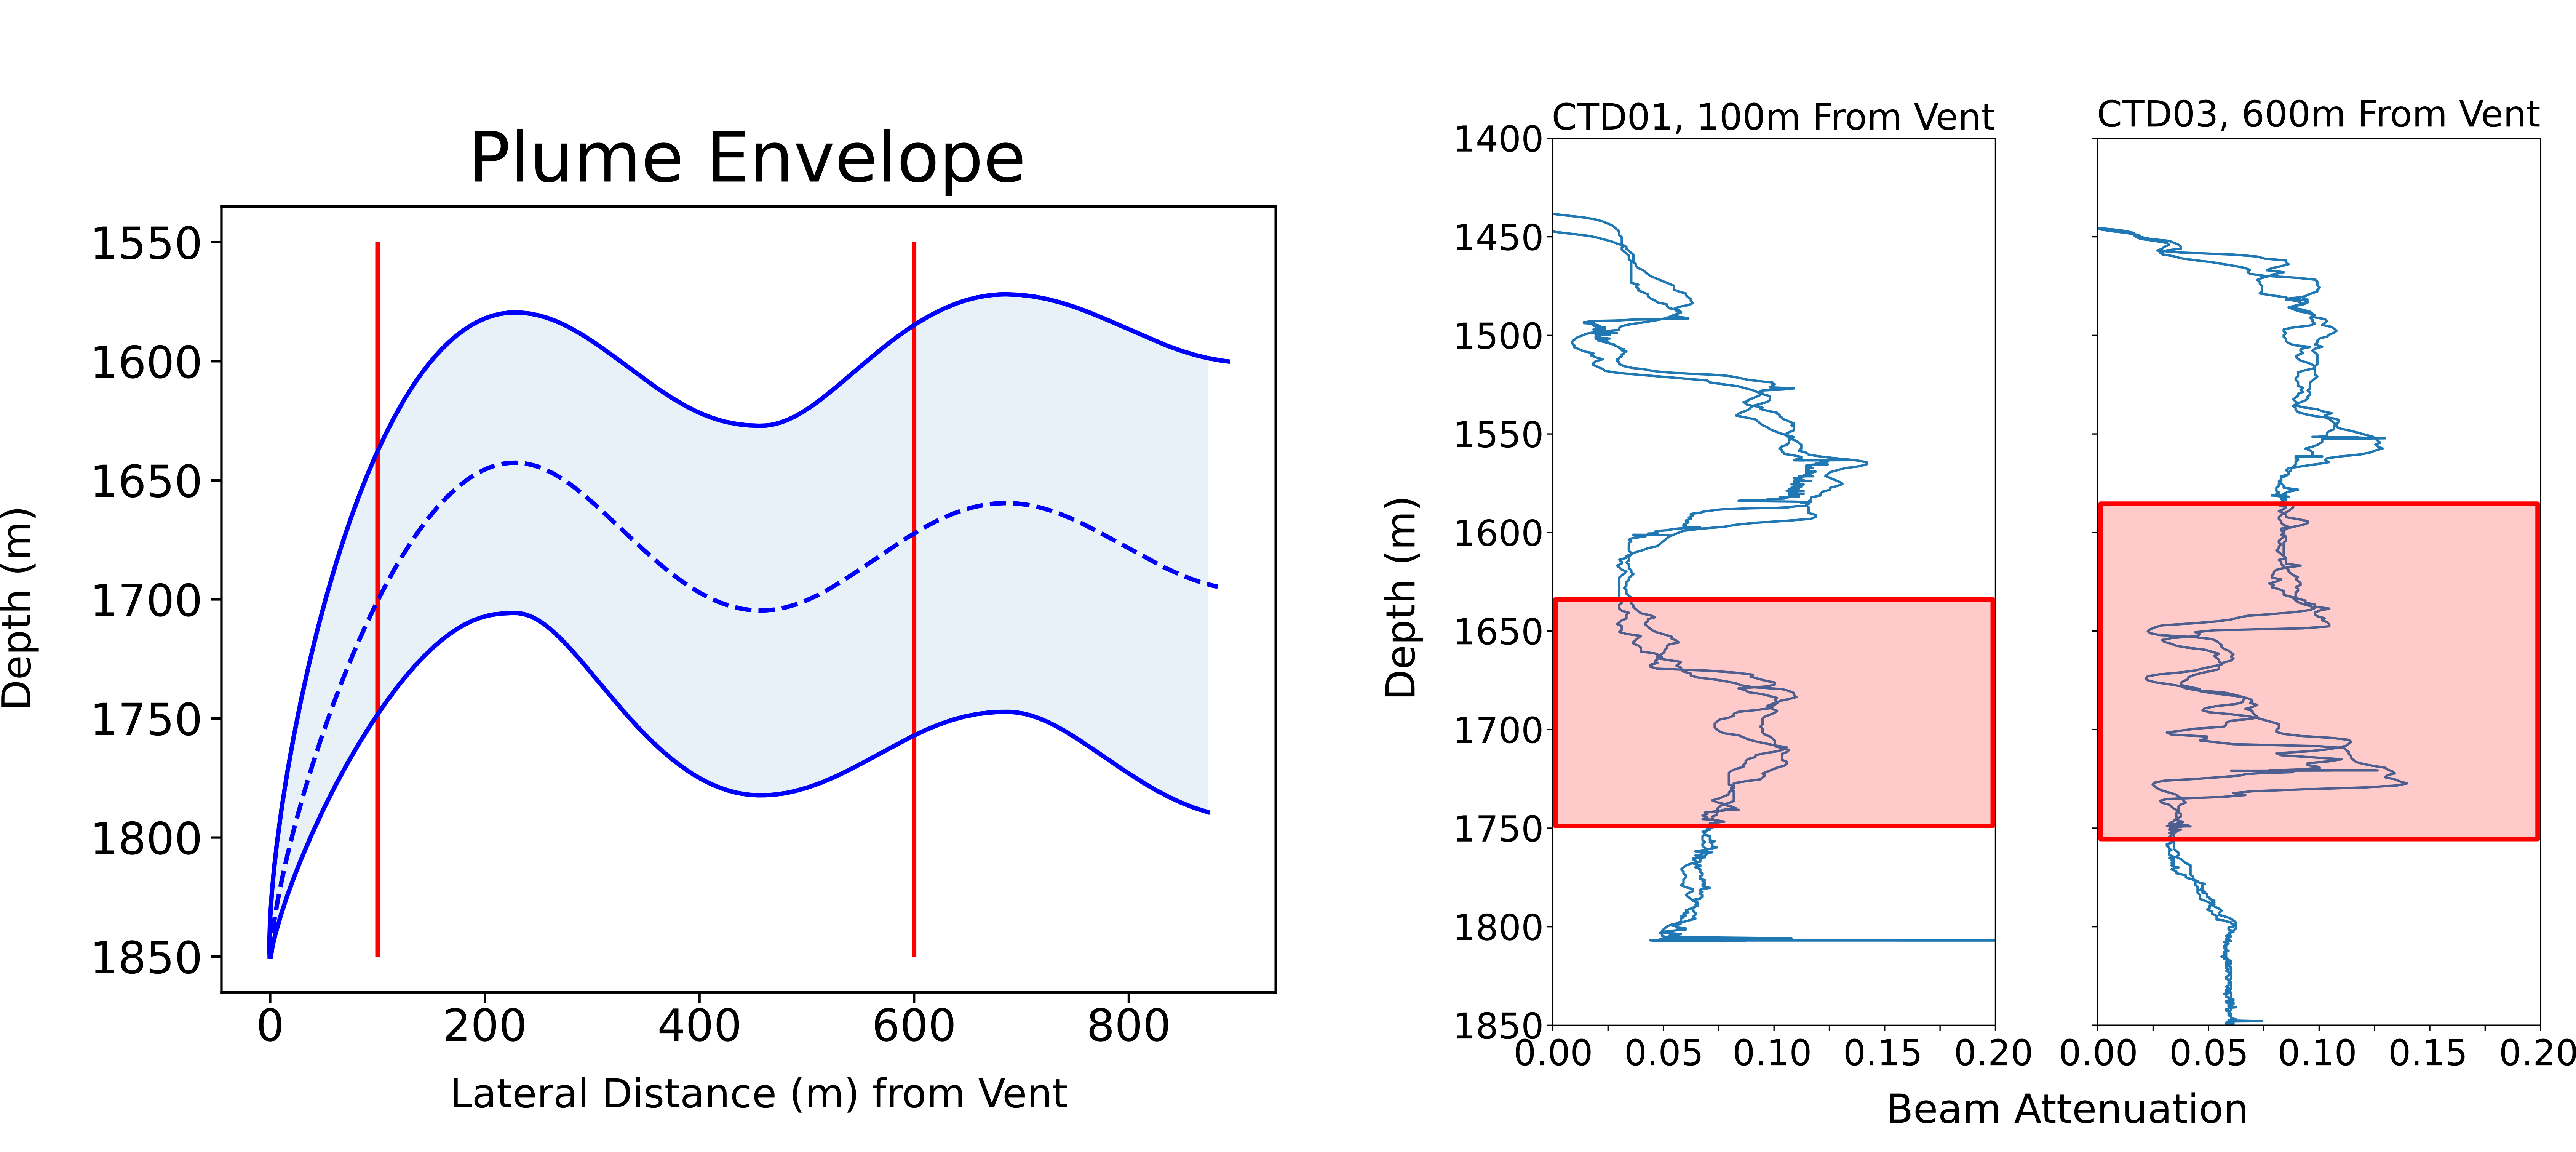
\includegraphics[width=1\columnwidth]{figures/field_validation.png}
    \caption[Validation of \PHUMES model trained at sea.]{\textbf{Validation of \PHUMES model trained at sea.} We compare the nominal plume estimate from \PHUMES trained on at-sea data and \Sentry observations with vertical transects of turbidity from shipboard rosette. The plume envelope is the average plume estimated by \PHUMES for a nominal crossflow of \SI{0.11}{\meter\per\second}. Vertical red lines mark \SI{100}{\meter} and \SI{600}{\meter} laterally from the originating vent, for which vertical CTD casts were conducted. The region that the model estimates containing the lowest plume intrusion in the water column is highlighted on the turbidity transects. There is agreement between the model estimate and the transect data on the location of this turbid layer.} 
    \label{fig:field_valid}
\end{figure}

\section{\PHUMES as a Science Model}
\label{sec:phumes_as_science}
We have shown that \PHUMES can learn explanatory models of the plume structure in a target environment through both simulation \cref{chap:field_results} and these field results which are useful for planning \PHORTEX trajectories. Here, we further investigate the utility of \PHUMES as a model for scientific inquiry, focusing on two key areas: investigation of energy flux, and descriptive summary of the neutrally-buoyant plume. \cref{fig:npb_flux} summarizes the results of the investigation.

\begin{figure}[h!]
    \centering
    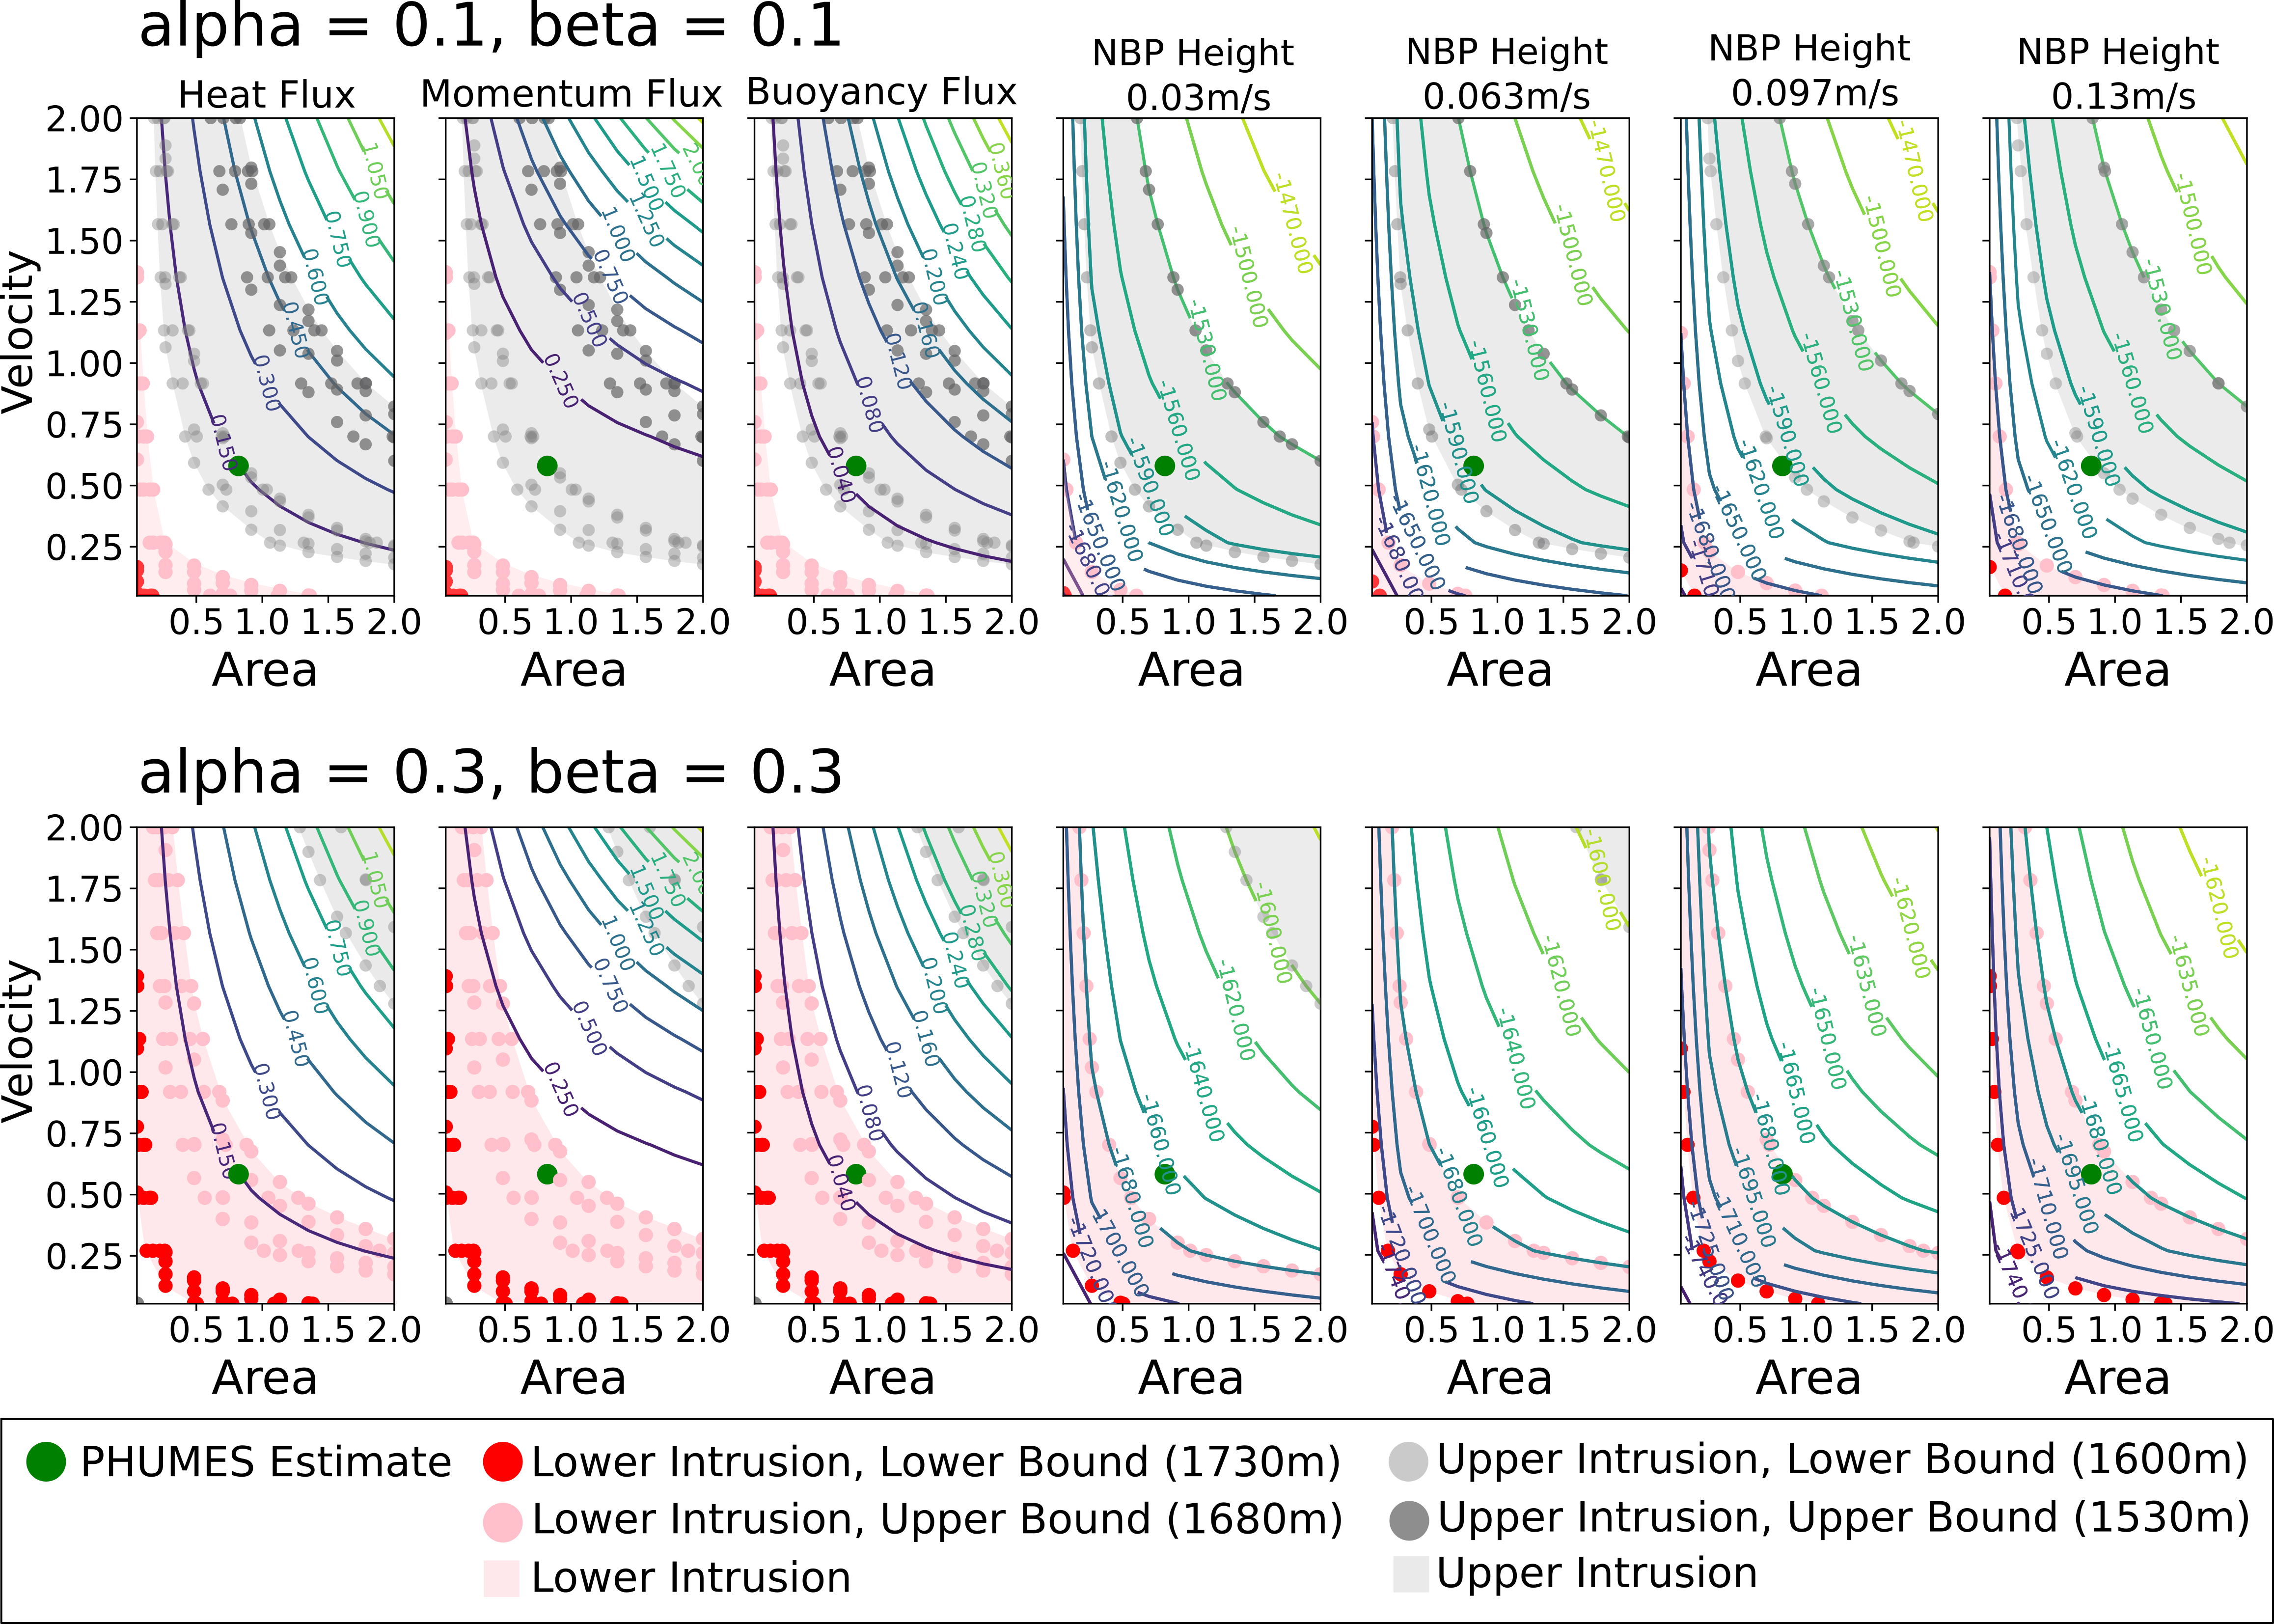
\includegraphics[width=1\columnwidth]{figures/flux_nbp.png}
    \caption[\PHUMES investigation of neutrally-buoyant plume height and energetic flux.]{\textbf{\PHUMES investigation of neutrally-buoyant plume height and energetic flux.} The heat, momentum, and buoyancy fluxes for a hypothetical vent are computed for different vent area and vent fluid exit velocity settings with two settings of mixing coefficients $\alpha$ and $\beta$ (first three columns, each row is an $\alpha$, $\beta$ setting). As mixing coefficient has no impact on flux estimation at a vent, the contours that describe the flux parameters are the same between the rows. Projected onto the flux plots are samples of velocity and area that align with particular neutrally-buoyant height depth values, selected from the vertical transects in \cref{fig:field_valid} that correspond with a deeper/lower intrusion (in pink, 1680-\SI{1730}{\meter}), and shallower/higher intrusion (in gray, 1530-\SI{1600}{\meter}). The samples are computed for different crossflow values, as specified by the 4 left-hand column plots. As entrainment values directly impact the neutrally-buoyant height computation and are related to the strength of crossflow, this leads to variation in the estimated velocity-area state space. The green dot in all plots represents the fixed velocity and area estimate learned by \PHUMES. In these plots, it is clear that a single fixed set of mixing coefficients may be insufficient to explain two distinctive inclusions, as the variation with current covers a relatively small margin for both coefficient settings. This implies that there may be alternative explanations of the presence of two intrusions: either mixing coefficients change in time (or could be modeled as such), or contributions from other plumes in the basin may be responsible for the overall vertical structure observed.}
    \label{fig:nbp_flux}
\end{figure}


As established in \cref{sec:field_rw}, one of the key reported metrics when studying hydrothermalism is the energetic characteristic of a venting source and the plume itself. Reports of estimated heat flux from hydrothermal vents vary; within the Guaymas Basin, a recent previous study has shown a wide range of hydrothermal energetic expressions within the soils of the basin\autocite{geilert2018formation}. In this study, specialized equipment was available to probe the soils directly to estimate diffusive flux. For chimney studies, access to similar equipment or ROVs can assist in directly measuring fluid exit velocity and area and the corresponding flux values can be constrained. While we had access to such equipment, the formation of the Guaymas chimneys---as many closely clustered, small orifices---make natural measurements of area and fluid velocity challenging, since complicated plume merging is taking place. Instead, it is more useful to understand the \emph{effective} area and fluid exit velocity, which will need to be inferred from water column data despite access to the venting sources. 

For water column observations, energy estimates are often computed using a stationary buoyant plume models, e.g.,~\cite{morton1956turbulent} or~\cite{speer1989model}, which do not take into account crossflow. To investigate how \PHUMES may be used for similar studies, we establish the relationship between the learned parameters $\x_c$ and $\x_p$, observations of the neutrally-buoyant layer intrusions in the water column, and energy fluxes (heat, momentum, and buoyancy). In general, flux at a vent orifice is computed using temperature, vent area, and vent fluid exit velocity; these values are agnostic to crossflow and mixing entrainment, as they are estimated to be the values immediately at the vent source. In \cref{fig:nbp_flux}, we show the contours which describe each of heat, buoyancy, and momentum flux with respect to a set of vent area and vent fluid exit velocity for a fixed temperature. As is evident, for any flux curve, there is a countably infinite set of velocity and area settings that could satisfy a given flux estimate. This leads to the notion of ``ill-posed'' inverse problems, as briefly discussed in \cref{sec:future}.

To begin to better explore the solution space, we can utilize more information, directly enabled by \PHUMES: crossflow. For the \PHUMES model, both crossflow and degree of mixing are linked to  the neutrally-buoyant plume height, which is observable by AUV or rosette transects. To understand the relationship between crossflow and neutrally-buoyant height, \cref{fig:nbp_flux} shows how estimates of fluid exit velocity and area can change for changing current magnitude and two particular settings of entrainment coefficients. Using the vertical transects in \cref{fig:field_valid} as a reference, two neutrally-buoyant intrusion layers can be identified---a lower intrusion at 1680-\SI{1730}{\meter} depth, and an upper intrusion at 1530-\SI{1600}{\meter} depth---and are mapped onto the plots for each current-entrainment setting. If we want to explain either intrusion with a fixed setting of exit velocity, area, and entrainment, we would likely want to pick a set of values that is always contained within the intrusion region colored on the plots. This would have a direct impact on the estimate of fluxes as well; all velocity-area regions across the different neutrally-buoyant height plots are projected onto the flux plots as well. We may use this projection to estimate a constant flux value that well describes the entire intrusion state space, or use the region to specify confidence bounds on a flux estimate.

What stands out in these plots, however, is that there is no combination of area, exit velocity, current, or entrainment coefficients that can fully describe the existence of \emph{both} intrusion layers. This is indicated by the failure of the pink and gray regions to overlap temporally for any fixed setting. If that overlap existed, it may strongly indicate a particular explanatory model of the vent characteristics; being able to tie complicated vertical structure to energetic contributions of a vent is a unique feature of this type of analysis \PHUMES enables. In absence of this overlap in the particular case of the Guaymas vent we study here, we can instead focus our attention to investigate other explanations for the presence of two intrusion layers: time/current-varying mixing coefficients (for instance, in these plots, temporal overlap between pink and gray regions could occur at low current magnitudes with small mixing coefficients and high current magnitudes with large mixing coefficients); the contribution of external hydrothermal expressions to the particular vent being studied (the ridge had multiple large chimneys at different depths, it is feasible then that the intrusion for a different chimney will manifest at a different place in the water column); or unmodeled forcing. To perform these investigations, physical water samples collected by the rosette could be analyzed from the different intrusion layers and their chemical ``fingerprints'' compared to determine whether they may have been generated by the same vents or to understand their relative age to one another. Continuous observations from \Sentry, as collected by \PHORTEX, could be used to more closely study the lower-intrusion distribution which may hint at possible unmodeled forces (e.g., the plume density is the same as background but still quite warm, which could lead to future density/buoyancy changes that manifest in a change in depth) or help to characterize the statistics of turbulent mixing observed (to inform the entrainment coefficients).

\PHUMES, in addition to providing a probability distribution over the vent and seawater characteristics, can also serve as a rich test-bed for investigating plume structure. Performing this type of analysis on a ship could assist in designing additional experiments or targeted sample collection that could directly drive at answering the new set of questions posed: how can two intrusions exist in the water column? what are the statistics of turbulence in the plume? what is the character of neutrally-buoyant plume waters relative to the ambient seawater? Answering these questions would not only drive at more accurate estimates of energetic flux, but also help inform where the shortcomings of the underlying analytical model may be, and over time and applied to new settings, these shortcomings could be addressed by formulating a new idealized model (just as \PHUMES is a response to consistent shortcomings in stationary buoyant rise models, today).


\section{Discussion and Future Work}
\label{sec:future}
There is a significant desire for embodied intelligence and assistive decision-making in environmental exploration and expeditionary science. \PHORTEX fundamentally relies on human expertise to inform the scientific models used within \PHUMES, generate useful reward functions, set trajectory primitives, and complete operationally safe and robust deployments while in the field. Relieving the burden on these human agents --- whether by creating aggregated data products or proposing multiple field missions with explanations --- could lead to significant gains in the short-term for expeditionary science tasks while robot technology matures. In the most simple case of this on the research cruise in this study, the real-time visualizer of acoustically transferred science data between \Sentry and the ship was sufficient for science experts to identify trends in robot performance with respect to the plume charting task. The capability of viewing real-time data, which to many academic and industrial roboticists may seem obvious or straightforward, is not yet pervasive or standard in the sciences or on state-of-the-art vessels and autonomous platforms. Research efforts on improving data infrastructure, data visualization, real-time signal processing, human decision-making, and supervised autonomy promise to be extremely impactful to the expeditionary sciences. 

In this chapter, we demonstrate that \PHORTEX scales and fits within a practical deployment-by-deployment mission in the field for hydrothermal plume charting. Data collected in the field demonstrated that \PHORTEX assists in collecting at least as many positive detections as science team experts, with gains in spatial utilization and temporal diversity; even on days old data. To implement \PHORTEX in the field required careful consideration of how to incorporate science data of opportunity, which is beyond the norm for planning under uncertainty problems and typical IPP solvers. The following section discusses several key areas for expanding IPP in similar ways for real field trails, and concludes with a discussion of how both \PHORTEX and \PHUMES, as modular frameworks, can serve as a methodological starting point for more general expeditionary science settings.

\paragraph{Compensating for Onboard Sensing Limitations of AUVs}
% comments on current inference and it being enabled by an external sensor
Leveraging historical or remote sensing equipment is well established for environmental studies in which satellite, fixed observatory, or historical observations are available for a human expert to use. However, as established in \cref{chap:opsatsea}, in oceanic environments, such observational equipment is not widely distributed and often needs to be independently deployed by a science team or by a robot explorer. In this study, we deployed a tiltmeter with ROV \emph{JASON} to compensate for one such shortcoming for observing the deep advecting currents in the basin. One of the key advantages of using the \PHUMES formulation, with a well-described analytical model at its core, is the ease by which many different types of information can be incorporated naturally and opportunistically. Black-box belief representations (e.g., neural learners, Gaussian Processes) could struggle to similarly take advantage of asynchronous, opportunistic data without intentionally planning for all possibilities or without considering a modular/hierarchical approach to formulating belief. Access to external equipment to a robot additionally invites advances in decision-making as well, as multiagent\autocite{salam2019adaptive,li2014multi,luo2018adaptive,ouyang2014multi} or task and motion-planning frameworks could be applied to expeditionary planning at large\footnote{e.g., \autocite{timmons2019automated}}. 

\paragraph{Scientific Implications of the Collected Data}
Tens of thousands of \emph{in situ} observations were collected in the four field dives that were executed in this study. These data can be directly used in external scientific frameworks for investigating hydrothermalism expressions in the Guaymas Basin. Most directly, \emph{in situ} observations of plume detections further than \SI{300}{\meter} will assist biochemists in mapping the fate of biologically digested chemicals and nutrients in hydrothermal fluids that rise through the water column. Coupled with physical bottle samples that the onboard science team collected, the \emph{Sentry} data from our dives will fill in the blanks between these sparse measurements. Given the rarity of scientific expeditions of the scale of cruise RR2107 and the ability to perform targeted sampling enabled by \PHORTEX, the data set collected is generally a contribution for the larger oceanographic community. In future work, we aim to directly expand on the investigation in \cref{sec:phumes_as_science} to estimate the rate of spread of fluid that intrudes into different strata of the water column, ultimately impacting estimates of the overall transport of particulates, chemicals, and nutrients into the larger basin ecosystem, and uniquely supported by the \PHUMES model.

\paragraph{Extending \PHORTEX and \PHUMES for Other Expeditionary Contexts}
% comments on how phortex and phumes can generalize
\PHORTEX and \PHUMES are formulated as modular frameworks, and in different expeditionary contexts each of the design decisions --- trajectory optimization scheme, definition of the reward function, and analytical model at the heart of \PHUMES --- could be replaced directly. \PHORTEX is formulated in this work as a deployment-by-deployment sequential decision-making framework that enables offline optimization of operationally-constrained trajectories. Fundamentally, this framework is general enough to extend to any robotic system which may not have access to adaptive behaviors, such as subsea AUVs and extraplanetary rovers. For online settings, \PHUMES is a model which can support the computation of information-theoretic reward functions and so online belief-based search\footnote{e.g., \autocite{flaspohler2019information, Arora2017, Sun2017, sunberg2018online}} common in adaptive sampling and IPP literature could be pursued instead. \PHUMES itself is a Bayesian inference model that centers around a particular choice for numerical simulator. To extend to other scientific settings, a different numerical simulator can be selected. This requires some initial knowledge of how a particular target environment may evolve; this knowledge could be partial (as in, only knowing that certain properties may be conserved), approximate (as is presented in this article as an idealized model of plume dynamics), or complete (as in, having a full-fidelity simulator of a target environment). Scientific expeditions in the ocean and other marine environments, as well as atmospheric studies, are particularly well-suited for formulation with \PHUMES to inform mobile robot trajectories given the wealth of numerical simulators which exist to describe these environments. 

\section{Conclusions}
\label{sec:field_conclusion}
Using mobile robots to perform science in the deep-sea is predicated upon both state-of-the-art autonomy systems, such as \PHORTEX, and on the effective use of resources within the operational constraints of an oceanographic research vessel. Beyond the core \PHORTEX method, this chapter presented a variety of technical and operational approaches to augment the performance of \PHORTEX and the science party during field deployments. For instance, we formulated a filtering technique which processed \Sentry data into a useful binary measurement of ``plume occupancy''. We additionally made use of non-robotic platforms and instruments to augment our learning procedure, which was enabled by using an underlying dynamical model in \PHUMES. \PHORTEX is modular and can be easily adapted to other domain-specific and expeditionary science tasks. The binary pseudo-sensor can be replaced with any discrete or continuous observation model; the scientific model leveraged within \PHUMES could be trivially swapped for another ODE or highly simplified PDE system (well-suited for e.g., ecological/population studies, fluid or thermal environments); and the reward function and trajectory optimization scheme can be modified based on the operational constraints of a target platform.

During a research cruise in November 2021, \PHORTEX was used in a sequence of four deployments of AUV \Sentry. The experimental results demonstrate that \PHORTEX can collect at least as many plume observations as surveys designed by expert human scientists and showed improved spatial and temporal diversity in samples for any given deployment, even when trained on days-old data. Through the field deployment, we demonstrated the first iterative offline planning technique for plume charting with deep-sea capable vehicles. The far-reaching impact of this demonstration is to assert that for the hundreds of deep sea vents only accessible by operationally restricted vehicles like \Sentry, strategic charting of complex spatiotemporal structure is within reach for future scientific studies. With this capability, novel questions about nutrient transport, water column ecosystems, and the fundamental structure of hydrothermal plumes can be more directly studied. In line with this ultimate goal, we demonstrated how \PHUMES can be used as an investigatory tool for plume structure and energetic characteristics, asserting several novel hypotheses for the formation of complex neutrally-buoyant intrusions in the water column at Guaymas Basin, and establishing a future path forward for additional analysis.
 